\documentclass[xcolor=dvipsnames]{beamer}
\usepackage{pgfpages}
\setbeameroption{show notes on second screen}

\usepackage[outline]{contour}
\usepackage{transparent}
\usepackage{pgfplots}
\usepackage[utf8]{inputenc}
\usepackage{multimedia}
\usepackage{graphicx}
\usetheme{Madrid}
\usepackage{amsmath,amssymb}
\usepackage{bm}
\usepackage[absolute,overlay]{textpos}
\usepackage{mathtools}
\usepackage{courier}
\usepackage{tikz}
\tikzstyle{every picture}+=[remember picture]
\usetikzlibrary{positioning}
\usetikzlibrary{math}
\usepackage{caption}
\usepackage{lmodern}
\beamertemplatenavigationsymbolsempty
\usefonttheme[onlymath]{serif}
\graphicspath{{./gfx/}}
\newcommand{\ppos}{q}
\newcommand{\pvel}{u}
\newcommand{\fpos}{r}
\newcommand{\fvel}{v}
\newcommand{\corr}{\text{corr}}
\newcommand{\dpr}{\text{\tiny DP}}
\newcommand{\qtd}{\text{\tiny q2D}}
\renewcommand{\vec}[1]{\bm{#1}}
\newcommand{\tens}[1]{\bm{\mathcal{#1}}}
\newcommand{\oper}[1]{\mathcal{#1}}
\newcommand{\uammd}{\gls{UAMMD}\xspace}
\newcommand{\gpu}{\gls{GPU}\xspace}
\newcommand{\dt}{\delta t}
\newcommand{\kT}{k_B T}
\newcommand{\sinc}{\textrm{sinc}}
\newcommand{\floor}{\textrm{floor}}
\newcommand{\near}{\textrm{near}}
\newcommand{\far}{\textrm{far}}
\newcommand{\half}{\frac{1}{2}}
\newcommand{\red}[1]{{\color{red}#1}}
\newcommand{\fou}[1]{\widehat{#1}}
\newcommand{\noise}{\widetilde{W}}

\newcommand{\executeiffilenewer}[3]{
  \ifnum
  \pdfstrcmp{\pdffilemoddate{#1}}{\pdffilemoddate{#2}}>0
  {\immediate\write18{#3}}
  \fi
}
\newcommand{\includesvg}[2][width=\columnwidth]{
  \executeiffilenewer{#2.svg}{#2.pdf}
  {inkscape -D #2.svg --export-type=pdf } %  --export-latex}
  %\def\svgwidth{#2}
  % \input{#1.pdf_tex}
  \includegraphics[#1]{#2.pdf}
}

\usepackage[absolute,overlay]{textpos}

\def\ucpp{uammd_cpp_lexer.py:UAMMDCppLexer -x}
\usepackage{tcolorbox}
\usepackage{xparse}
\tcbuselibrary{breakable,minted,xparse,skins,listings}
\usemintedstyle{default}
\setminted[\ucpp]{ %
  linenos=false,             % Line numbers
  autogobble=true,          % Automatically remove common white space
  fontsize=\small,
  breaklines
}
\AtBeginDocument{
  \newtcblisting{code2}[2][]{
    colback=white,
    colbacktitle=white,
    coltitle=black,
    pad at break*=0mm,
    listing only,
    listing engine=minted,
    listing remove caption=true,
    title={~#1},
    minted language=\ucpp,
    enhanced jigsaw,
    minipage boxed title,
    attach boxed title to bottom center={xshift=0mm,yshift=-1mm},
    boxed title style={size=small, blanker},
    center title,
    #2
  }
}
\tcbsetforeverylayer{autoparskip}


\makeatother
\setbeamertemplate{footline}
{
  \leavevmode%
  \hbox{%
  \begin{beamercolorbox}[wd=.4\paperwidth,ht=2.25ex,dp=1ex,center]{author in head/foot}%
    \usebeamerfont{author in head/foot}\insertshortauthor
  \end{beamercolorbox}%
  \begin{beamercolorbox}[wd=.6\paperwidth,ht=2.25ex,dp=1ex,center]{title in head/foot}%
    \usebeamerfont{title in head/foot}\insertshorttitle\hspace*{3em}
    \insertframenumber{} / \inserttotalframenumber\hspace*{1ex}
  \end{beamercolorbox}}%
  \vskip0pt%
}
\makeatletter
\makeatletter
\newcommand{\howmany}[2][subsection]{%
  \begingroup
  \@namedef{the#1}{\arabic{#1}}%
  \addtocounter{#1}{\m@ne}%
  \refstepcounter{#1}%
  \label{#2}%
  \endgroup}
\makeatother

\title{Complex fluids in the GPU era}
\subtitle{Algorithms and simulations}
\author{Raul P. Pelaez}

\institute{Universidad Autónoma de Madrid}
\date{\today}

%\captionsetup[figure]{font=small,skip=0pt}
\usepackage[export]{adjustbox}
\setbeamertemplate{itemize subitem}{$\rightarrow$}
\newcounter{framesectioncounter}
\AddToHook{cmd/section/before}{\setcounter{framesectioncounter}{0}}
\pdfmapfile{-mpfonts.map}
\usepackage{lmodern}
\everymath{\displaystyle}
\begin{document}


\begin{frame}
  \titlepage
  \centering
\small  Supervisor: Rafael Delgado-Buscalioni
  \begin{figure}
    \centering
    
\includegraphics[width=0.25\linewidth]{UAMlogo}
  \end{figure}
  \note{This is a GPU. A powerful hardware with a unique programming model. Harvesting its tremendous raw power requires developing algorithms and software specifically tailored for it. My work during these past years has been devoted to exploiting the GPU for the simulation of complex fluids. Now, before we continue, let me give you a summary of this talk. }
\end{frame}

%\section{This thesis main contributions}

\section{Introduction}

\begin{frame}
  \frametitle{Talk outline}
  \only<1>{\tableofcontents[
    sectionstyle=show/shaded,
    subsectionstyle=show/show/hide,
    subsubsectionstyle=show/show/show/hide
    ]
  }
  \only<2>{
    \tableofcontents[
    sectionstyle=show/show,
    subsectionstyle=hide/hide/hide,
    subsubsectionstyle=hide/hide/hide/hide
    ]
  }
  \note{
    \begin{itemize}
    \item I will start by introducing what complex fluids are, with an overview of the numerical and mathematical machinery we use to simulate them in a computer.
    \item Then I will talk about the main algorithmic hardships that arise in this field and I will focus on how to solve some of them with a GPU.
    \item Part of my contributions consist on the developing of new GPU-enabled algorithms for hydrodynamics and electrostatics in confined geometries, which I will also introduce.
    \item The main contribution of my work lies in UAMMD, a GPU software framework for complex fluids that I built from scratch during these years and that includes, among others, all the algorithms and solvers that I will mention in this talk.
      \item I will then end with some conclusions.
    \end{itemize}
  }
\end{frame}



%\begin{frame}
%  \frametitle{Outline}
%  \begin{itemize}
%  \item UAMMD's functionalities
%  \item Particle-based and grid based
%  \item Code structure
%    \begin{itemize}
%    \item open-source
%    \item adaptable
%    \item ...
%    \end{itemize}
%  \end{itemize}
%\end{frame}
%

\subsection{Complex fluids}
\begin{frame}
  \frametitle{Complex fluids}
\centering \Large  The coexistence between a liquid and solid phase
  \begin{figure}
    \centering
    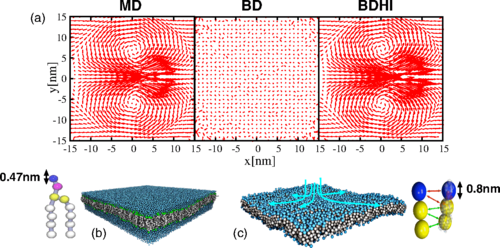
\includegraphics[width=0.5\linewidth]{membrane}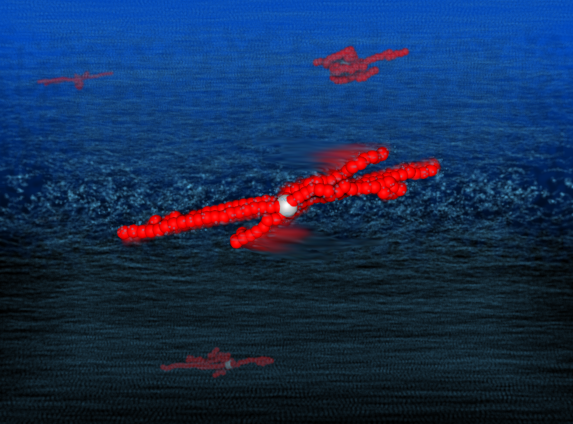
\includegraphics[width=0.2\linewidth]{star}
    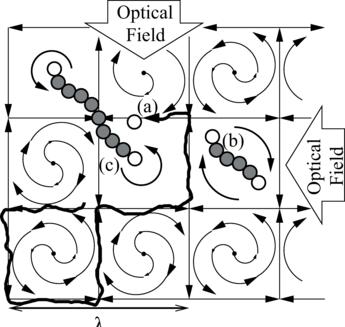
\includegraphics[width=0.2\linewidth]{optofluidics}\\
    {\fontsize{4.5}{12} \selectfont [{\bf Panzuela, S. and Delgado-Buscalioni, R.} PRL 2018.]  -  [{\bf Raul P. Pelaez and Delgado-Buscalioni, R.} Macromolecules 2020]    -   [{\bf  Mel\'endez, M.} et. al. PRE 2019.]}\\
    \only<1>{\movie[autostart,loop,poster,showcontrols=true,width=0.3\linewidth]{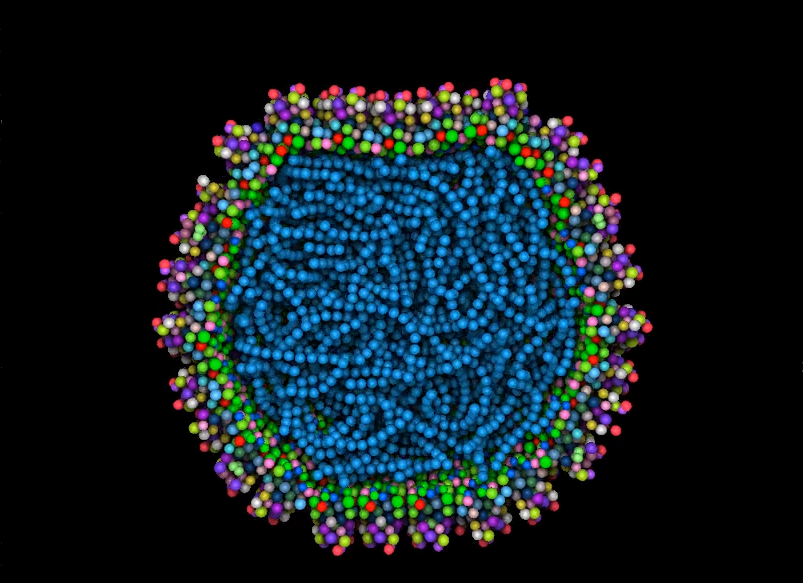
\includegraphics[width=0.3\linewidth]{virus_scr.png}}{gfx/virus.mp4}}%
    \only<2>{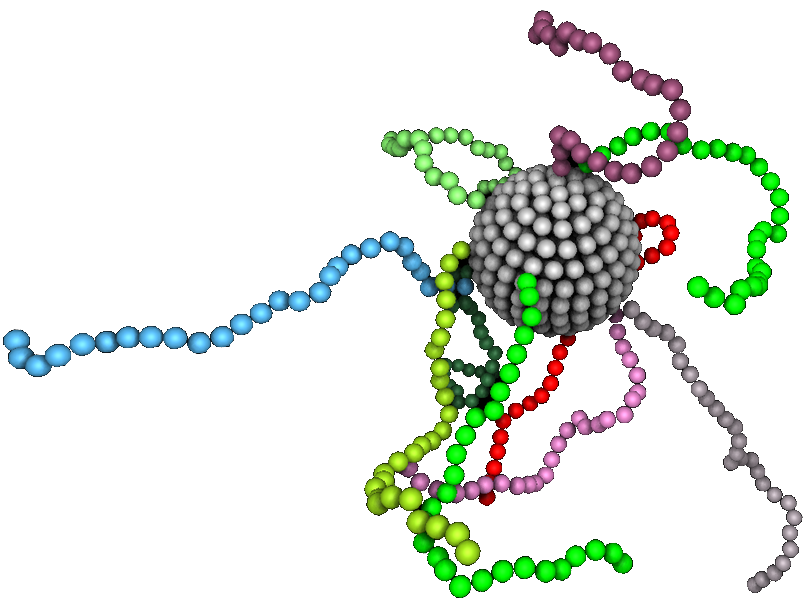
\includegraphics[width=0.235\linewidth]{lipostrandspablo.png}}%
    \movie[autostart,loop,poster,showcontrols=true,width=0.3\linewidth]{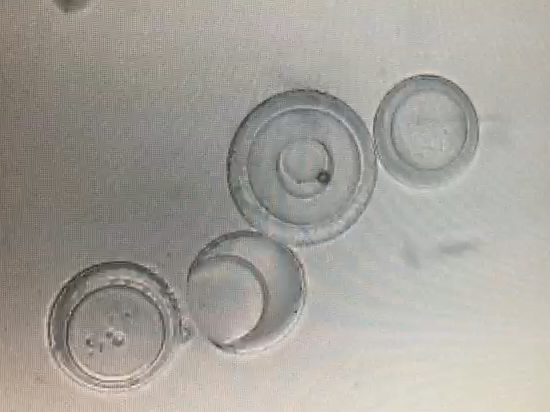
\includegraphics[width=0.3\linewidth]{rots.png}}{gfx/rots.mp4}%
    \only<1>{%
      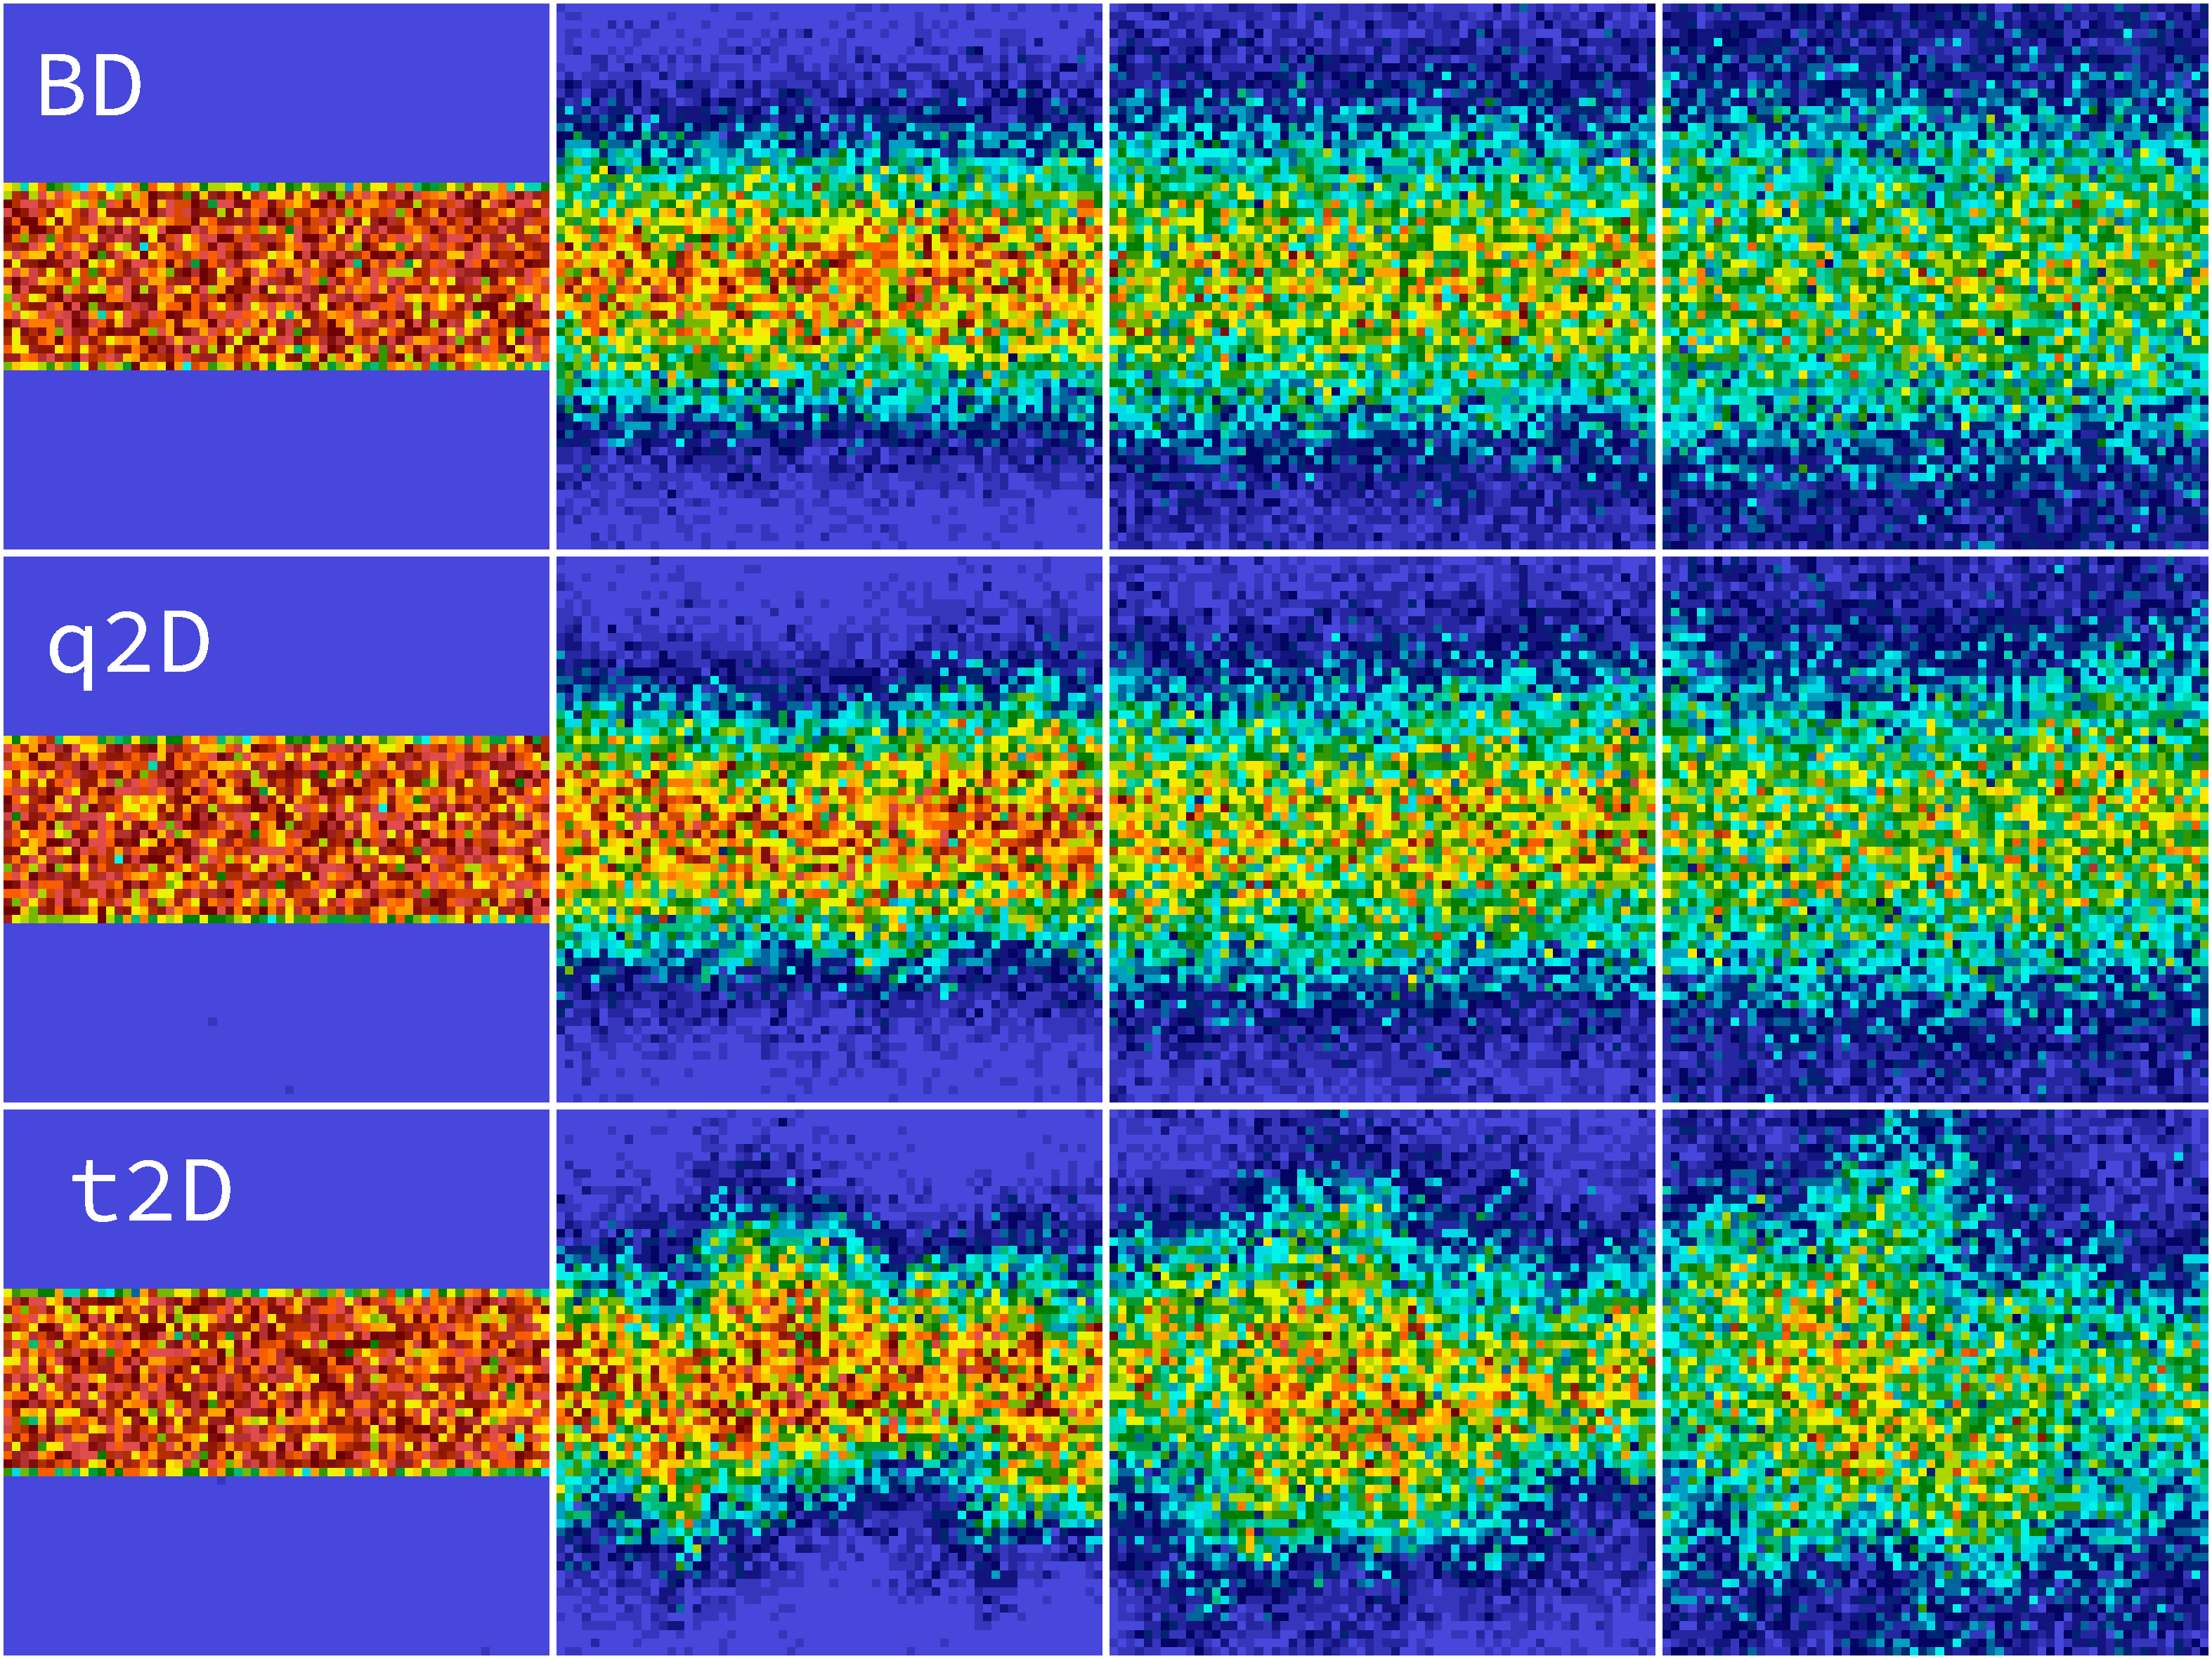
\includegraphics[width=0.3\linewidth]{q2Dcolorstripe}\\
      {\fontsize{4.5}{12} \selectfont [Courtesy of Pablo Ibañez] ------------ [Courtesy of Berta Tinao] -------------- [{\bf Raul P. Pelaez} et. al. JSTAT 2018.]}%
    }
    \only<2>{%
      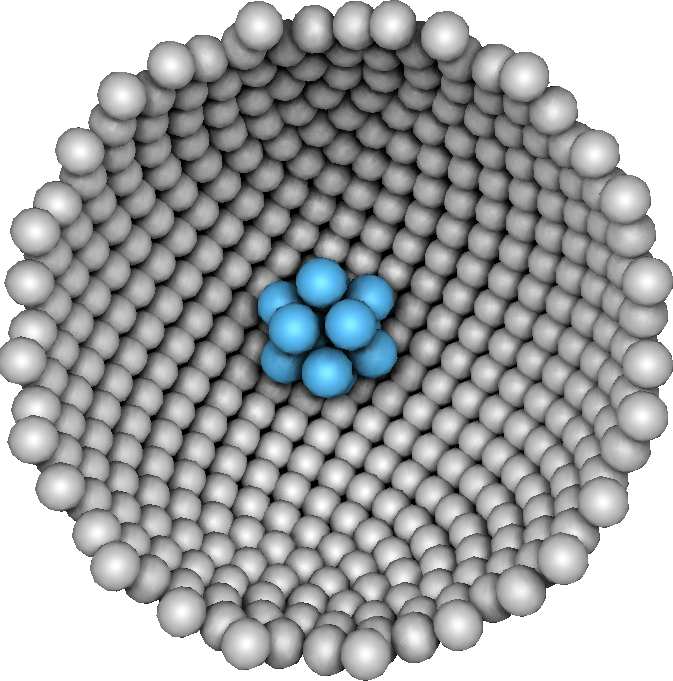
\includegraphics[width=0.22\linewidth]{mnppablo.png}\\
      {\fontsize{4.5}{12} \selectfont [Courtesy of Pablo Palacios] ------------------------ [Courtesy of Berta Tinao] ----------------------------------------- [Courtesy of Pablo Palacios]}
    }
  \end{figure}
  \note<1>{
    \scriptsize
    \begin{itemize}
    \item I showed you what a GPU is at the start. In order to understand the rest of the title you also need to know what a complex fluid is.
    \item Although its definition is a little more general, we understand a complex fluids as the coexistence between a solid and a liquid phase. And note that with solid, we usually mean soft, such as a colloidal particle or a cell's lipidic membrane.
    \item This broad definition encloses a wide variety of systems, many times of biological nature. In this slide I show you a bunch of examples, all of them taken from past and ongoing works in our group.
    \item Starting up we can see coarse-grained representations of a lipid bilayer, a star polymer in a shear flow, a nano dumbell swimming and spinning in a fluid under optically-induced vortexes. A virus capsid, filled with a particular protein, which is being pressed by an AFM tip (the video is not long enough, but the virus ends up exploding under the pressure). Next we have a group of lipidic vesicles, one of them contains a ferromagnetic particle that, when subject to a magnetic field, spins the vesicle. This allows to somewhat control the locomotion of the vesicles. The final picture shows the diffusion of the concentration of a colloidal suspension under strong two-dimensional confinement in different regimes.
    \end{itemize}    
  }  
  \note<2>{
    \begin{itemize}
    \item Here, the figure to the right shows a model of the rotating vesicles a member of group, Pablo, is studying now, in part using the tools and algorithms that I will shortly introduce.
    \item Pablo has also studied other kinds of magnetic nanoparticles.
    \item These examples showcase enormous span of the spatio-temporal scales associated with complex fluids. Sometimes we need to focus on single polymers, or describe a single polymer in detail. Other times we want to model vesicles that are almost visible to the naked eye.
    \end{itemize}
  }
\end{frame}


\subsubsection{Numerical techniques}
\begin{frame}
  \frametitle{Complex fluids}
  \framesubtitle{The spatio-temporal landscape of numerical techniques.}
  \begin{figure}
    \centering
    \begin{tikzpicture}
      \only<1-5>{\node[anchor=south west, inner sep=0] (image) {\includesvg[width=0.8\linewidth]{gfx/landscape}};}
      \begin{scope}[shift={(image.south west)},x={(image.south east)},y={(image.north west)}]
        %\draw foreach \xy in {0,0.1,...,1.001}{(\xy,0) -- node[pos=0,below]{\pgfmathprintnumber{\xy}} (\xy,1)(0,\xy) -- node[pos=0,left]{\pgfmathprintnumber{\xy}} (1,\xy)};
        \only<2>{\filldraw[red, opacity=0.6] (0.12,1) rectangle (0.5,0.07) node[midway] (A) {};\node[above=50pt of A, black]{\contourlength{1pt}\contour{white}{\textbf{Fully Lagrangian}}};}
        \only<4>{\filldraw[blue, opacity=0.6] (0.5,1) rectangle (0.72,0.07) node[midway] (A) {};\node[below=40pt of A, black, align=left]{\contourlength{1pt}\contour{white}{\textbf{Eulerian}}\\\contourlength{1pt}\contour{white}{\textbf{Lagrangian}}};}
        \only<3>{\filldraw[green, opacity=0.6] (0.72,1) rectangle (1,0.07) node[midway] (A) {};\node[above=50pt of A, black]{\contourlength{1pt}\contour{white}{\textbf{Fully Eulerian}}};}
      \end{scope}
    \end{tikzpicture}
    \caption{Figure courtesy of Rafael Delgado-Buscalioni.}
  \end{figure}
  \note<1>{
    \begin{itemize}
    \item The modeling and simulation of complex fluids thus greatly exceeds the scope of the typical computation window. Speaking in terms of this numerical landscape we cannot specialize in a single window. If we want to model a complex fluid, we must take into account sizes ranging from nanometers to meters and times going from nanoseconds to seconds. And even then, we are restricted to a narrow-ish area of the lanscape, being unable to, for instance, simulate a nanometer-sized system for several hours of physical time.
    \item I claim that my software, UAMMD, covers the whole range of the complex-fluid domain, and I hope to convince you during this talk that this is true.
    \item Anyway, countless numerical and mathematical techniques exists depending on our window of interest, and their naming scheme can sometimes be a little obtuse.      
    \end{itemize}
  }
  \note<2>{
    \begin{itemize}
    \item Broadly speaking, we can categorize the landscape into three families of methods.
    \item When studying small systems, we usually choose a fully Lagrangian scheme, meaning that we track the evolution of individual particles, or markers.      
    \end{itemize}
  }
  \note<3>{
    \begin{itemize}
    \item On the contrary, when focusing on macroscopic systems we usually choose a fully Eulerian description, where we loose track of individual particles and instead describe continuous fields.      
    \end{itemize}
  }
  \note<4>{
    \begin{itemize}
    \item In the middle, in what we call the mesoscale, there is a mixed domain of Eulerian-Lagrangian methods, where we describe both a group of particles and continuous fields that are somehow coupled.
    \item This is the realm of hydrodynamics, where most of the examples I showed you take place.
    \item I would like to point out now that my algorithmic contributions lie in this regime.
    \end{itemize}
  }
  \note<5>{
    \begin{itemize}
    \item Let us focus in the red area, covering an, in principle, disparate range of descriptions all owning to complex fluids.
    \item If we start at the atomic scale and want to climb up the spatio-temporal scale of modeling we can make use of coarse graining techniques, where we want to somehow average out the fast degrees-of-freedom that are of no interest to us. For instance, if we are describing a submarine running under the sea (by all means a complex fluid) we really want to leave the individual water atoms out of our description.
    \end{itemize}
    }
\end{frame}

\subsubsection{Coarse-grained levels of description}
\begin{frame}
  \frametitle{Complex fluids}
  \framesubtitle{Usual levels of coarse-grained description}
  \begin{figure}
    \centering
    \includesvg[width=0.55\linewidth]{gfx/multiscale}
  \end{figure}
  \note{
    In particular, we can cover the whole range using the following four levels of coarse-grained description. Going through them will help us understand how we can design a framework that covers them all.
    }
\end{frame}


\begin{frame}[t]
  \frametitle{Complex fluids}
  \framesubtitle{Usual levels of coarse-grained description}
  \begin{columns}[T]
    \begin{column}{0.5\linewidth}
        \begin{tikzpicture}
          \node[anchor = south west, inner sep = 0] (image) {\includesvg[width=\linewidth]{gfx/multiscale}};
          \begin{scope}[shift={(image.south west)},x={(image.south east)},y={(image.north west)}]
            %Draw a overlaying grid to easily see where the rectangles must be, this can be commented out in the final version
%            \draw foreach \xy in {0,0.1,...,1.001}{
%            (\xy,0) -- node[pos=0,below]{\pgfmathprintnumber{\xy}} (\xy,1)
%            (0,\xy) -- node[pos=0,left]{\pgfmathprintnumber{\xy}} (1,\xy)};
            \foreach[count=\i] \mypath in {
              {(0,1) rectangle (0.48,0.55)},
              {(0.48,1) rectangle (1.0,0.55)},
              {(0,0.55) rectangle (0.48,0)},
              {(0.48,0.55) rectangle (1,0)},
              {(0,1) rectangle (1,0)},
              {(0,1) rectangle (1,0)}
            }{
              \filldraw<\i>[white,opacity=0.9,even odd rule] (0,0) rectangle (1,1) \mypath;
            }
          \end{scope}
        \end{tikzpicture}
      \end{column}
      \begin{column}{0.45\linewidth}
      \begin{center}
        \textbf{Relevant variables:}
      \end{center}
      \begin{itemize}
      \item<1-> $\vec{q}_i$: Position of particle $i$.
      \item<1-3,5-> $\vec{u}_i$: Velocity of particle $i$.
      \item<3,5-> $\xi(\vec{q}_{ij})$: Friction kernel.
      \item<2,5-> $\vec{v}(\vec{r},t)$: Fluid velocity field.
      \item<4-> $M(\vec{q}_{ij})$: Mobility tensor.
      \end{itemize}
      \centering      
      \only<1-4>{\textbf{Typical timescale:}\newline}
      \only<1>{$\tau \sim 10^{-12}s$}
      \only<2>{$\tau \sim 10^{-\{9-6\}}s$}
      \only<3>{$\tau \sim 10^{-5}s$}
      \only<4>{$\tau \sim 10^{-3}s$}
      \only<5->{\textbf{Timescale range:}\newline $\tau \sim [10^{-12}, 10^{-3}]s$}
    \end{column}
  \end{columns}
  \only<1>{\begin{textblock*}{0.5\linewidth}(0.05\linewidth, 0.55\paperheight)}
  \only<2>{\begin{textblock*}{0.53\linewidth}(0.05\linewidth, 0.49\paperheight)}
  \only<3>{\begin{textblock*}{0.5\linewidth}(0.05\linewidth, 0.2\paperheight)}
  \only<4,5>{\begin{textblock*}{0.5\linewidth}(0.05\linewidth, 0.17\paperheight)}
  \only<6>{\begin{textblock*}{0.99\linewidth}(0.04\linewidth,0.23\paperheight)}
    \begin{block}<1-4>{
        \only<1>{Molecular Dynamics (MD)}
        \only<2>{Immersed Boundary Method (IBM)}
        \only<3>{Langevin Dynamics (LD)}
        \only<4>{Brownian Dynamics (BD)}
      }{$$\only<1>{%
          \begin{aligned}
            m\ddot{\vec{\ppos}} &= \vec{F}\\
            \vec{\pvel} &= \dot{\vec{\ppos}}
          \end{aligned}
        }%
      \only<2>{%
          \begin{aligned}
            &\rho\partial_t\vec{\fvel} = -\vec{\partial}_{\vec{\fpos}}\cdot \tens{\sigma} + \vec{f} + \text{fluct}\\
            \int_{V_p}\vec{f}d\vec{\fpos} &= \vec{F}_i\quad\text{and}\quad \vec{u}_i = \int_{V_p}\vec{\fvel}d\vec{\fpos}
          \end{aligned}%
       }%
      \only<3>{m d\vec{\pvel} = \vec{F}dt - \xi\vec{\pvel}dt +  \sqrt{2\xi\kT}\vec{\noise}}%
      \only<4>{%
          \begin{aligned}%
            d\vec{\ppos} =& \tens{M}\vec{F}dt + \sqrt{2\kT\tens{M}}d\vec{\noise}\\%
                          &+ \kT\vec{\partial}_{\vec{\ppos}}\cdot\tens{M}dt.%
          \end{aligned}%
        }%
        $$}
    \end{block}
    \begin{alertblock}<6>{\centering \Large We always have}
      \centering \Large
      Interacting \emph{particles} with a \emph{state} that \emph{evolves}.
    \end{alertblock}
  \end{textblock*}
  \centering
  \only<1>{
    Supervector notation $\vec{q} := \{\vec{q}_1,\dots,\vec{q}_N\}$
  }
  \only<2>{
    $\partial_t := \frac{\partial}{\partial t} \rightarrow \vec{\partial}_{\vec{r}} := \nabla := \left(\partial_x,\partial_y,\partial_z\right) $ 
  }
  \only<3>{
    $\vec{\noise}$: Wienner increments, $\mathcal{N}(0,dt)$
  }
  \only<4>{
    $d\vec{\noise}$: Wienner increments, $\mathcal{N}(0,dt)$
  }

  \note<1-5>{
    \begin{itemize}
      \only<1>{
      \item At the lowest level (the most detailed one) we find the microscopic level, where we need to describe the positions and velocities of every atom (or small group of atoms) involved in the system. This includes every water molecule conforming the fluid in addition to the particles embedded in it. The Newton equations of motion govern this level, where the inter-particle forces are of atomic origin. Notice that this is a fully Lagrangian description.
      \item The typical timescale is given by the fast-moving fluid particles.
      \item BTW, note that I am using the so-called supervector notation here, where a symbol without a subindex often refers to the list of all related quantities. As opposed to, for instance, $\vec{q}_i$, which refers to a specific particle called ``i''. I will abuse this notation throughout this talk, so beware!.
      }
      \only<2>{
        \footnotesize
      \item Going up we have the hydrodynamic level, where the individual degrees of freedom of the fluid particles are lost and we are left, instead, with a continuous velocity field representing them. The math tells us that when we do this, we must reintroduce the lost degrees-of-freedom as thermal fluctuations.
      \item Thus this is an Eulerian-Lagrangian formalism and is governed by the Navier-Stokes equations describing the fluid. A fluid which exists in a two-way coupling with a group of embedded particles.
      \item This coupling is far from trivial, but in essence it consists of the particles communicating their forces to the fluid via a force density and, in return, the particles following the fluid by sampling its surrounding velocity. $V_p$ here is the volume of a particle (whatever that means).
      \item The typical timescale is given by the speed of sound of the fluid as well as its vorticity. In other words, how fast it communicates information.
      }
      \only<3>{
      \item When particles move so slowly compared to the solvent characteristic times, hydrodynamic interactions,
        which were previously mediated by a velocity field, are effectively instantaneous. We call this the Langevin level.
      \item We eliminate the fluid velocity, transforming it into a friction kernel (and of course, fluctuations). Typically, this friction kernel will be defined pairwise, although it could simply be a constant, or depend on the entire particle configuration.
      \item Only the positions and momenta of the particles remain as relevant variables (taking us back to a Lagrangian description once again),
        which obey a Langevin equation.
      \item The characteristic decorrelation time of the particle's velocities governs this scale.
      }
      \only<4>{
      \item At some point in our upwards journey, the particle positions change slowly enough that their velocity decorrelates
        effectively instantaneously, thus inertia can be disregarded and positions are the only relevant variable.
      \item Here, the friction kernel has morphed into a mobility tensor (which is the inverse of a friction) and is typically dependent on the position of every particle. Although once again, it might be a simple constant, for instance if we neglect hydrodynamic interactions.
      \item The dynamics are described by the Brownian Dynamics equations of motion (an over-damped Langevin equation).
      \item The diffusion time of the particles dominates this level.
      }
      \only<5>{
      \item Let me show you again all the levels of description, which overall allows us to describe a really wide timescale range.
      \item Now, there is a not-so-hidden theme here that has allowed me to design a software framework encasing all of this.
        Have you noticed it?
      }
    \end{itemize}
  }
  \note<6>{
    \begin{itemize}
    \item In all instances, we can vaguely describe the situation as a ``group of interacting \emph{particles} with a \emph{state} that \emph{evolves}''. Whatever a particle, its state or how it evolves mean in each case. And it is worth noticing this definition also includes other schemes I have not mentioned, such as a Monte Carlo simulation.
    \item Note that even when a continuous field is present, we can interpret that it only exists as a proxy to communicate the particles. Think of a particle that moves a fluid, which in turns moves the rest of the particles (and in fact this movement reflects back to original particle and so on and so forth).
    \end{itemize}
  }
\end{frame}

\section{Elements of a complex fluid simulation}
\begin{frame}
  \frametitle{Talk outline}
  \tableofcontents[
  sectionstyle=show/shaded,
  subsectionstyle=show/show/hide,
  subsubsectionstyle=show/show/show/hide
  ]
  \note{
    \begin{itemize}
    \item Later, I will show you how I leveraged this sentence to create UAMMD, but first I want to discuss the other side of a complex fluid simulation. We have seen about the kind of solvers that we can use to unravel the dynamics of particles for simulations in different spatio-temporal windows, but there is a long way between having equations for the solvers and writing a GPU code for them.
    \item Besides the mathematical hardships we may face along the way (and we will see some of them later on), we have to tame the algorithmic complexity of the interactions, them being either those arising from the dynamics (such as hydrodynamics) or from particle-particle couplings (such as sterics or electrostatics).
    \item In this regard, we basically encounter the same set of three problems again and again, which I would like to go through in this next section.
    \end{itemize}
  }
\end{frame}


% \subsection{Computational Challenges}



\begin{frame}
  \frametitle{Computational challenges}
  \setbeamercovered{transparent=40}
  \begin{columns}[T]
    \begin{column}{0.6\linewidth}
      \begin{enumerate}
        \Large
      \item Short range interactions
      \item<1> Long range interactions
      \item<1> Particle-grid coupling
      \end{enumerate}
      \begin{overlayarea}{\linewidth}{0.5\paperheight}
        \only<2>{\centering Example: Lennard-Jones potential
          $$U_{LJ}(r) = 
            \begin{cases}
              4 \epsilon \left[ \left(\frac{\sigma}{r}\right)^{12} - \left( \frac{\sigma}{r}\right)^6 \right] & r<r_c\\
              0 & r\ge r_c
            \end{cases}$$
          }
      \end{overlayarea}
    \end{column}
    \begin{column}{0.4\linewidth}
      \only<2>{
        \begin{figure}
          \centering                 
          \includesvg[width=\linewidth]{gfx/nlist}
        \end{figure}
      }
    \end{column}
  \end{columns}
  \note{
    \begin{itemize}
      \only<1>{\item We have three types of problems to solve. Short- and long-range interactions and Eulerian-Lagrangian coupling.}
      \item The first one arises, for instance, with steric interactions, which are cut-off after a certain distance.
      \item And the problem here lies in finding the particles inside the radius of action of the red particle checking the least amount of black particles possible.
    \end{itemize}
  }
\end{frame}

\subsection{Short range}
\begin{frame}
  \frametitle{Short range interactions}
  \framesubtitle{Neighbour lists}
  \begin{figure}
    \centering
    \includesvg[width=0.8\linewidth]{gfx/sketchUAMMD_nlist}%    
  \end{figure}
  \note{
    \scriptsize
    \begin{itemize}
    \item The canonical solution for this is using a neighbour list.
    \item In the GPU we find three main strategies for it. Each of them typically excelling in different situations.
    \item The cell list works by binning the domain and identifying the bin of each particle. Then, the neighbours of the black particle are found by visiting the neighbouring bins. The orange particles are false positives.
    \item When the cell list fails, for instance when there are large concentration disparities, we can use tree-based lists. In particular, UAMMD implements the so-called Linear Bounding Volume Hierarchy algorithm, which partitions the domain in a hierarchical fashion, with boxes encasing increasingly large boxes.
    \item In any case, we leverage the Verlet strategy, which consists of using any of the two to elaborate an interaction list with an artificially enlarged cut of radius. This way, the list can be reused for several steps, as long as the particles do not diffuse a lot.
    \end{itemize}
    }
\end{frame}

\begin{frame} 
  \frametitle{Short range interactions}
  \framesubtitle{Neighbour lists: Performance}
  \begin{block}{Example: Lennard-Jones potential, $r_c=2.5\sigma$ and $\varepsilon = kT$.}
    $$U_{LJ}(r) = 
    \begin{cases}
      4 \varepsilon \left[ \left(\frac{\sigma}{r}\right)^{12} - \left( \frac{\sigma}{r}\right)^6 \right] & r<r_c\\
      0 & r\ge r_c
    \end{cases}$$
  \end{block}
  \includegraphics[width=0.49\linewidth]{nlistperf_dens1}
  \includegraphics[width=0.49\linewidth]{nlistperf_dens0.1}
  \begin{center}
    \scriptsize Ran with a single RTX2080Ti GPU.
  \end{center}
  \note{
    \begin{itemize}
    \item Let me show you how these compare in UAMMD's implementations.
    \item In this example I am showing timings for the computation of the forces for a Lennard Jonnes liquid at two different densities. We are seeing time per step versus the number of particles as I make the system bigger. There is a lot to unpack in this figure but sadly not a lot of time, so the take away message here is that they are all somewhat similar and they all present linear scaling. It is also worth noting that we can update 10 million particles at around 100 times a second.
    \end{itemize}
  }
\end{frame}

\subsection{Long range}
\begin{frame}
  \frametitle{Computational challenges}
  \begin{columns}[T]
    \begin{column}{0.6\linewidth}
      \begin{enumerate}
        \Large
      \item {\transparent{0.4} Short range interactions}
      \item Long range interactions
      \item {\transparent{0.4} Particle-grid coupling}
      \end{enumerate}
      \begin{overlayarea}{\linewidth}{0.5\paperheight}
        \only<2->{\centering Electrostatics:
          $$U_{\text{Coulomb}}(r) = \frac{1}{4\pi \varepsilon_0}\frac{Q_iQ_j}{r} $$
          \centering Hydrodynamics:
          $$\tens{O}(\vec{r}) = \frac{1}{8\pi\eta r}\left(\mathbb{I} - \frac{\vec{r}\otimes\vec{r}}{r^2}\right)$$
        }
      \end{overlayarea}
    \end{column}
    \begin{column}{0.4\linewidth}
      \begin{figure}
        \centering                 
        \only<2>{\includesvg[width=\linewidth]{gfx/nbodycon}}%
        \only<3>{\includesvg[width=\linewidth]{gfx/pbc}}%
      \end{figure}
    \end{column}
  \end{columns}
  \note<1>{The next challenge is long, or infinitely, ranged interactions.}
  \note<2>{
    \begin{itemize}
    \item Such is the case, for instance, of electrostatics and hydrodynamics, interactions decaying just as the inverse of distance.
    \item We could go ahead and check every pair of particles in the system. An quite GPU-friendly algorithm, alas with a high operation count.
    \item And that is not taking into account periodic boundary conditions, which would take the operation count of this naive approach to infinity.
    \end{itemize}
  }
\end{frame}


\begin{frame}
  \frametitle{Long range interactions}
  \begin{columns}[T]
    \begin{column}{0.4\linewidth}
      \begin{itemize}
      \item Brute force
      \item Spectral methods
        \onslide*<3->{%
          \begin{itemize}
          \item FFT:\\ cuFFT (library calls)
          \item Coupling:\\ Hand made%
          \end{itemize}
        }%
      \item {\small\transparent{0.5} Hierarchical/multigrid methods}
      \end{itemize}
    \end{column}
    \begin{column}{0.6\linewidth}%
      \begin{overlayarea}{\linewidth}{0.5\paperheight}
      \only<1>{\includesvg[width=0.7\linewidth]{gfx/nbodycon}}%
      \only<2->{\includesvg[width=\linewidth]{gfx/fftpibm}}%
      \end{overlayarea}
    \end{column}%
  \end{columns}
  \note<1>{
    \begin{itemize}
    \item Luckily, we have some alternatives beside brute-forcing it that scale linearly with the number of particles, even with periodic boundary conditions.
    \item Mainly, we can distinguish between spectral and hierarchical or multigrid methods. I have left the second type out of this talk, since I have not focused on this family of algorithms during my phd.
    \end{itemize}
  }
  \note<2,3>{
    \begin{itemize}
    \item Spectral methods are based on the Fast Fourier transform, which happens to be incredibly efficient on the GPU.
    \item We are dealing with particles, though, so we need a Non Uniform Fourier transform. Which involves transforming our Lagrangian markers into an Eulerian field.
    \end{itemize}
    }
\end{frame}






\subsection{Particle-grid coupling}

\begin{frame}
  \frametitle{Computational challenges}
  \setbeamercovered{transparent=40}
  \begin{columns}[T]
    \begin{column}{0.6\linewidth}
      \begin{enumerate}
        \Large
      \item {\transparent{0.4} Short range interactions}
      \item {\transparent{0.4} Long range interactions}
      \item Particle-grid coupling
      \end{enumerate}
      \begin{overlayarea}{\linewidth}{0.5\paperheight}
        \only<2->{
          \centering Spreading ($\oper{S}$):
          $$\vec{f}(\vec{r}) = \oper{S}(\vec{r})\vec{F} := \sum_i \vec{F}_i\delta_a(\vec{r}-\vec{q}_i)$$
          \only<3->{{$\delta_a(\vec{r}) := \phi(r_x)\phi(r_y)\phi(r_z)\rightarrow$ Smeared delta}\newline\newline}
        }
        \only<4>{
          \centering Interpolation ($\oper{J}$):
          $$\vec{u}_i = \oper{J}_{\vec{q}_i}\vec{v}(\vec{r}) = \int \vec{v}(\vec{r})\delta_a(\vec{r}-\vec{q}_i)d\vec{r}$$
        }
        \only<5>{
          \centering Interpolation ($\oper{J}$):
          $$\vec{u}_i = \oper{J}_{\vec{q}_i}\vec{v}(\vec{r}) \approx \sum_n \vec{v}_n\delta_a(\vec{r}_n-\vec{q}_i)h^3$$
        }        
      \end{overlayarea}
    \end{column}
    \begin{column}{0.4\linewidth}
      \onslide*<2->{
      \begin{figure}
        \centering                 
        \only<2>{\includesvg[width=\linewidth]{gfx/ibm_spread}}%
        \only<3>{          
          \resizebox{\linewidth}{!}{
            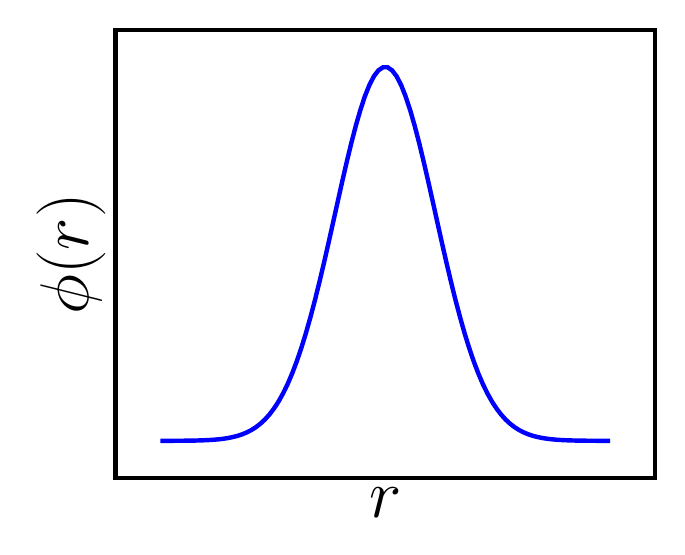
\begin{tikzpicture}
              \begin{axis}[ticks=none,samples=100,ylabel={\Huge $\phi(r)$},xlabel={\Huge $r$}, xlabel near ticks, ylabel near ticks, axis line style=ultra thick]
                \addplot[blue, ultra thick, domain=-1:1] {exp(-x^2*10)};
              \end{axis}
            \end{tikzpicture}
          }
        }
        \only<4,5>{\includesvg[width=\linewidth]{gfx/ibm_interp}}%
      \end{figure}
    }
    \only<3>{\centering Example: $\phi(r) \propto e^{-\frac{r^2}{2\sigma^2}}$}
    \end{column}
  \end{columns}
  \setbeamercovered{transparent=0}
  \onslide<2>{{\footnotesize Supervector notation $\vec{F} := \{\vec{F}_1,\dots,\vec{F}_N\}$}}
  \note<1>{
    \begin{itemize}
    \item And this takes us to the third challenge, which is the communication between particles and a grid.
    \end{itemize}
  }
  \note<2>{
    \begin{itemize}
    \item We can use this coupling for a number of things. For instance, to transform a series of forces, F, acting on a group of particles into a force density discretized on a grid. We call this operation spreading.
    \item Note that, for a given location, we must sum over all particles, since there might be overlap, i.e, several markers contributing to the same position.
    \end{itemize}
  }
  \note<3>{
    \begin{itemize}
    \item This communication is mediated via a compactly-supported bell-shaped kernel.
    \end{itemize}
  }
  \note<4>{
    \begin{itemize}
    \item We often need the inverse operation as well, that is averaging a discrete field at the positions of a series of particles.
    \end{itemize}
  }
  \note<5>{
    \begin{itemize}
    \item  For instance, to compute the velocity of a certain particle based on a velocity field defined on a grid.
    \item  The non-uniform Fourier transform is the basis all the Eulerian-Lagrangian algorithms presented in my work, and thus it is worth describing in more detail how we can efficiently perform the spreading and interpolation operations in a GPU.
    \end{itemize}
  }
\end{frame}

\begin{frame}
  \frametitle{Particle-grid coupling}
  \framesubtitle{GPU thread geometry}
  \includesvg[width=0.8\linewidth]{gfx/cudablocks}\\
  \onslide<2->{
    \centering
    \Large Special considerations:
    \begin{itemize}
    \item<2-> Massively parallel
    \item<3-> Single Instruction Multiple Data (SIMD)
    \item<4-> Mostly memory-bandwidth bound
    \end{itemize}
  }
  \note{
    \begin{itemize}
    \item First, we need to understand a little bit more about how GPUs work.
    \item Broadly speaking, in a CPU, we typically have dozens of powerful workers, or threads, that, while sharing the same underlying memory pool, largely function as individual processors.
    \item<2-> On the contrary, a GPU offers thousands of threads, which are grouped into blocks of a few hundreds.
    \item<3-> And there is a caveat, all threads in a block must all perform the same operation at the same time. 
    \item<4> This operation can be applied to different data, but GPU payloads tend to be bottlenecked by memory operations.
    \item<4> To aid with this, we have several memory spaces available. The slow access global memory is accessible by threads in every block, while shared memory is fast but only available to the threads inside the same block and only when the GPU is running a job.
    \end{itemize}
    }
\end{frame}

\begin{frame}
  \frametitle{Particle-grid coupling}
  \framesubtitle{GPU-friendly algorithm}
  \begin{columns}
    \begin{column}{0.6\linewidth}
      \begin{itemize}
      \item {\color{ForestGreen} $b_i$}: Block assigned to particle $i$.
      \item {\color{red} $t_j$}: Thread $j\in [0:N_b)$ of block $i$, assigned to grid point $n$.
      \end{itemize}
      \begin{block}<2->{\textbf{Spreading:} $\vec{f}_n = \sum_i \vec{F}_i\delta_a(\vec{r}_n-\vec{q}_i)$}
        $t_j\rightarrow$ write to $\vec{f}_n$ \alert<4>{atomically}.
      \end{block}
      \begin{block}<3->{\textbf{Interpolation:} $\vec{u}_i = \sum_n \vec{v}_n\delta_a(\vec{r}_n-\vec{q}_i)h^3$}
        \textbf{1.} $t_j\rightarrow$ gather from $\vec{v}_n$.\\
        \textbf{2.} $t_{\{0\dots 9\}}$ reduce into $\vec{u}_i$.
      \end{block}
    \end{column}
    \begin{column}{0.4\linewidth}
      \includesvg[width=\linewidth]{gfx/ibm_algo}
    \end{column}
  \end{columns}
  \note<1>{
    \begin{itemize}
    \item Naturally, this is just the tip of the iceberg, but hopefully enough to get us going.
    \item Let me get back to spreading an interpolation now.
    \item My strategy consists on assigning a block of threads to each particle, so that each thread in the block takes care of a different nearby grid point. We can take advantage of several threads working on the same particle and perform some computations only once per block. For instance, precomputing the kernel and storing it in shared memory.
    \end{itemize}
  }
  \note<2>{
    \begin{itemize}
    \item For spreading, a block per particle means that each thread computes the contribution of a particle and adds it to a single grid point atomically (given that other threads, for other particles, might be attempting the same thing at the same time).
    \end{itemize}
  }
  \note<3>{
    \begin{itemize}
    \item Interpolation is inherently more efficient, since we only have to read the grid information. Each thread computes the contribution of a different nearby grid point. After summing all of them only one thread needs to write the final result for the particle.
    \end{itemize}
  }

\end{frame}

\begin{frame}
  \frametitle{Particle-grid coupling}
  \framesubtitle{Spreading: Performance of a random distribution}
  \centering
  \includegraphics[width=0.6\linewidth]{gfx/ibm_comp_dens1_2080ti}\\
  \begin{minipage}{0.4\linewidth}
    \begin{exampleblock}{Largest number of particles}
      \centering
      $N=512^3 \approx 1.3\cdot 10^8$
    \end{exampleblock} 
  \end{minipage}
  \note{
    \scriptsize
    \begin{itemize}
    \item Let us see how efficient this strategy is. This is the time it takes to spread one particle as we increase the number of particles in a random distribution. And this has two important consequences: First a lot of overlapping can happen and second, there is no correlation between a particle's physical position and its location in GPU memory.
    \item Here BPP represents the block-per-particle algorithm I described. TPP is a naive thread-per-particle implementation. SM is a recent sophisticated alternative that assigns a block to a piece of the domain instead of a particle, trying to avoid atomic operations.
    \item I used a random distribution because I wanted to test something out. In theory a random distribution could potentially reduce atomic overlapping at the cost of a worse memory access pattern. If atomics are so bad then this should be worth it.
    \item My claim here is that GPU atomics are so efficient nowadays that we do not really have to worry about them.
    \item If I am right, a more cache-friendly memory pattern should be more important than avoiding atomics. So let us turn things around.
    \end{itemize}
    }
  % \begin{columns}[T]
%    \begin{column}{0.4\linewidth}
%    \end{column}
%    \begin{column}{0.6\linewidth}
%
%    \end{column}
%  \end{columns}
\end{frame}

\begin{frame}
  \frametitle{Increasing data locality}
  \only<+>{\includesvg[width=0.8\linewidth]{gfx/celllist0}}%
  \only<+>{\includesvg[width=0.8\linewidth]{gfx/celllist1}}%
  \only<+>{\includesvg[width=0.8\linewidth]{gfx/celllist2}}%
  \note{
    \begin{itemize}
    \only<1>{\item Let us sort the particles so that particles close in space are also close in memory.}
    \only<1>{\item The numbers above these particles represent their location in memory. Random.}
    \only<2>{\item But if we virtually bin the domain...}
    \only<3>{\item ... we can assign a hash to each particle based on its position. If we are smart about this hash, like this curve here that represents an increasing value of the hash, when we sort the particles based on it we will end up with a better access pattern. Note that now particles are ordered following the red curve.}
    \end{itemize}
    }
\end{frame}

\begin{frame}
  \frametitle{Particle-grid coupling}
  \framesubtitle{Performance}
  \centering
  \begin{tikzpicture}    
    \begin{scope}
      \draw node[anchor = west, inner sep = 0] (image) {\includegraphics[width=0.49\linewidth]{gfx/ibm_comp_dens1_sorted_2080ti}};
    \end{scope}
    \draw node [above] (text) at (image.north) {\huge Sorted};
    \begin{scope}
      \draw node[anchor = east, inner sep = 0] (image2) {\includegraphics[width=0.49\linewidth]{gfx/ibm_comp_dens1_2080ti}};
    \end{scope}
    \draw node [above] (text2) at (image2.north) {\huge Unsorted};
  \end{tikzpicture}\\
  \begin{minipage}{0.4\linewidth}
    \begin{exampleblock}{Largest number of particles}
      \centering
      $N=512^3 \approx 1.3\cdot 10^8$
    \end{exampleblock}
  \end{minipage}
  \note{
    \begin{itemize}
    \item Now, does this work? It turns out it does! and by a lot. The black being quasi horizontal means that we have achieved linear scaling, and with quite a good timing.
    \item In this case simplicity beats complexity and we can conclude that GPU atomics are a really powerful tool.
    \end{itemize}
  }
\end{frame}

\section{New doubly periodic solvers}
\begin{frame}
  \frametitle{Talk outline}
  \tableofcontents[
  sectionstyle=show/shaded,
  subsectionstyle=show/show/hide,
  subsubsectionstyle=show/show/show/hide
  ]
  \note{
    \begin{itemize}
    \item Let us put what we just learned to practice, by discussing some algorithms, developed during my phd for computing hydrodynamics and electrostatics in confined geometries. Both of them, long-ranged interactions.
    \item I will start with two algorithms for hydrodynamics.
    \end{itemize}
  }
\end{frame}

\begin{frame}
  \frametitle{Hydrodynamics in confined geometries}
  \framesubtitle{New algorithms for Brownian Dynamics with Hydrodynamic Interactions (BDHI)}
    \begin{figure}
    \centering
    \includesvg[width=0.55\linewidth]{gfx/multiscale}
  \end{figure}
  \note{
    \begin{itemize}
    \item I am going to focus on the Smoluchowski level SOMETHING MORE
    \end{itemize}
  }
\end{frame}

\begin{frame}
  \frametitle{Complex fluids}
  \framesubtitle{The spatio-temporal landscape of numerical techniques.}
  \begin{figure}
    \centering    
    \begin{tikzpicture}
      \node[anchor=south west, inner sep=0] (image) {\includesvg[width=0.8\linewidth]{gfx/landscape}};
      \onslide<2>{
        \begin{scope}[shift={(image.south west)},x={(image.south east)},y={(image.north west)}]
        %\draw foreach \xy in {0,0.1,...,1.001}{(\xy,0) -- node[pos=0,below]{\pgfmathprintnumber{\xy}} (\xy,1)(0,\xy) -- node[pos=0,left]{\pgfmathprintnumber{\xy}} (1,\xy)};
%        \only<2>{\filldraw[red, opacity=0.6] (0.12,1) rectangle (0.5,0.07) node[midway] (A) {};\node[above=50pt of A, black]{\contourlength{1pt}\contour{white}{\textbf{Fully Lagrangian}}};}
        \filldraw[blue, opacity=0.6] (0.5,1) rectangle (0.72,0.07) node[midway] (A) {};\node[below=40pt of A, black, align=left]{\contourlength{1pt}\contour{white}{\textbf{Eulerian}}\\\contourlength{1pt}\contour{white}{\textbf{Lagrangian}}};
%        \only<3>{\filldraw[green, opacity=0.6] (0.72,1) rectangle (1,0.07) node[midway] (A) {};\node[above=50pt of A, black]{\contourlength{1pt}\contour{white}{\textbf{Fully Eulerian}}};}
      \end{scope}
      }
    \end{tikzpicture}
    \caption{Figure courtesy of Rafael Delgado-Buscalioni.}
  \end{figure}
  \note{
    \begin{itemize}
    \item We will require techniques that mix both continuous fields and particles.
    \end{itemize}
    }
\end{frame}


\subsection{Hydrodynamics}
\begin{frame}
  \frametitle{Smoluchowski level}
  \framesubtitle{Brownian Dynamics with Hydrodynamics Interactions (BDHI)}
  \Large
  \begin{equation*}
    d\vec{\ppos} = \tens{M}\vec{F}dt + \sqrt{2\kT\tens{M}}d\vec{\noise}
    + \kT\vec{\partial}_{\vec{\ppos}}\cdot\tens{M}dt.
  \end{equation*}
  \vspace*{10pt}
  \begin{overlayarea}{\linewidth}{0.6\paperheight}
    \only<1-3>{
      \begin{itemize}
      \item<1-> $\tens{M}(\vec{\ppos})$:\\
        Mobility tensor. Configuration- and BC-dependent
      \item<2-> $d\vec{\noise}$: Brownian motion
      \item<3-> $\kT\vec{\partial}_{\vec{\ppos}}\cdot\tens{M}dt$:\\
        Thermal drift. Zero depending on the BCs
      \end{itemize}
    }
    \only<4->{
      \centering \textbf{Problems}
      \vspace*{10pt}
      \begin{itemize}        
        \setlength\itemsep{10pt}
      \item<5-> $\tens{M}\vec{F}$: Matrix-vector multiplication is $O(N^2)$
      \item<6-> $\sqrt{\tens{M}}$: Quite expensive in general. $O(N^{[2.25-3]})$
      \item<7-> $\tens{M}$ might be unknown/not analytical.
      \end{itemize}
    }
  \end{overlayarea}
  \note{
    \begin{itemize}
    \only<1>{\item The Smoluchowski level is governed by the Brownian Dynamics equations of motion. Which can be written as follows.}
    \only<1>{\item Here, M is a Mobility tensor, which in general is a symmetric matrix with elements for all pairs of particles.}
    \only<2>{\item We also have some thermal fluctuations.}
    \only<3>{\item And in general, a so-called thermal drift term that is luckily, many times null.}
    \only<4>{\item Sadly, applying this equation directly is far from trivial in most instances.}
    \only<5>{\item For starters, applying the mobility involves multiplying a 3Nx3N matrix and a 3N vector.}
    \only<6>{\item Moreover, we need to compute the square root of the mobility, whatever that means.}
    \only<7>{\item And to make things worse, many times we do not even have an expression for the mobility. Which is an object that emerges from macroscopic hydrodynamics.
    \item Instead of using this equation, we can arrive at the same dynamics by solving the Stokes equations coupled with particles. This opens the way to a family of Eulerian-Lagrangian algorithms, our specialty.}
    \end{itemize}
    }
\end{frame}


\begin{frame}
  \frametitle{Hydrodynamics}
  %\only<1-4>{\framesubtitle{Incompressible Navier-Stokes equations}}
  %\only<4->{\framesubtitle{Fluctuating Incompressible Navier-Stokes equations}}
  %\only<8->{\framesubtitle{Fluctuating Stokes equations}}
  \framesubtitle{\only<6->{Fluctuating} Stokes equations}
  \begin{equation*}
    \label{eq:navierstokes}
    \begin{aligned}
      %\onslide<1-7>{\overbrace{\underbrace{\rho\partial_t{\vec{\fvel}}}_{\text{time}} +\underbrace{\rho\nabla\cdot (\vec{\fvel}\otimes\vec{\fvel})}_{\text{convection}}}^{\text{fluid inertia}}}
      \onslide<2->{\overbrace{-\eta \nabla^2\vec{\fvel}}^{\text{momentum diffusion}}}
      \onslide<3->{&= \underbrace{-\nabla \pi}_{\text{internal stress}}}
      \onslide<4->{+ \underbrace{\tilde{\vec{f}}}_{\text{\parbox{2cm}{\centering external stress}}}}\\
      \onslide<5->{\nabla\cdot\vec{\fvel} &= 0\quad\mathllap{\underbrace{\phantom{\nabla\cdot\vec{\fvel} = 0}}_{\text{incompressibility}}}}
    \end{aligned}
  \end{equation*}
  \onslide<6->{
    \begin{equation*}
      \tilde{\vec{f}}(\vec{r}) := \underbrace{\vec{f}(\vec{r})}_{\text{external forces}} + \overbrace{\nabla\cdot \mathcal{Z}}^{\text{thermal noise}}
    \end{equation*}
  }
  \onslide<7->{
    \begin{equation*}
      \label{eq:navierstkesnoise}
      \begin{aligned}
        &  \langle \mathcal Z_{ij}\rangle = 0\\
        &  \langle \mathcal Z_{ik}(\vec{\fpos},t)\mathcal Z_{jm}(\vec{\fpos}',t')\rangle = 2\kT\eta(\delta_{ij}\delta_{km} + \delta_{im}\delta_{kj})\delta(\vec{\fpos}-\vec{\fpos}')\delta(t-t')
      \end{aligned}
    \end{equation*}
  }
  \note{
    \begin{itemize}
    \item The Stokes equations are the inertia-less version of the Incompressible Navier Stokes equations. And can be understood as a balance between the momentum diffusion of the fluid and the stress that it is subjected to.
    \item This stress comes from its internal pressure and any external stress, such as forces and thermal fluctuations.
    \item Here, Z is a tensor that is designed to comply with fluctuation-dissipation balance.
    \end{itemize}
  }
\end{frame}

\begin{frame}
  \frametitle{Hydrodynamics}
  \framesubtitle{Fluctuating Stokes equations}
  \begin{columns}[T]
    \begin{column}{0.34\linewidth}
      \begin{block}{Stokes equations}
        $%
        \begin{aligned}%
          \nabla \pi - \eta \nabla^2\vec{\fvel} &=  \vec{f} + \nabla\cdot \mathcal{Z}\\
          \nabla\cdot\vec{\fvel} &= 0%
        \end{aligned}
        $%
      \end{block}
      \onslide<2->{
        \begin{minipage}{\linewidth}
          \begin{block}{Fluid forcing}
            \centering $\vec{f}(\vec{r}) = \oper{S}(\vec{r})\vec{F}$
          \end{block}
          \begin{block}{Particle velocity}
            \centering $\vec{u}_i = \oper{J}_{\vec{q}_i}\vec{v}(\vec{r})$
          \end{block}
        \end{minipage}
      }
      \end{column}
      \begin{column}{0.63\linewidth}
        \onslide<3->{
          {
            \begin{center}
              \huge \textbf{Green formalism}
            \end{center}
          }
          \centering $\vec{v} = \oper{G}\tilde{\vec{f}}
          \onslide<4->{
            :=\int{\oper{G}(\vec{r}, \vec{r}^\prime)\tilde{\vec{f}}(\vec{r}) d\vec{r}^\prime}
          }$ %\left(\oper{S}\vec{F} + \nabla\cdot\mathcal{Z}\right)$$
          \onslide<5->{
            \begin{block}{Force Coupling Method (FCM)}
              \centering $\frac{d\vec{q}_i}{dt} = \vec{u}_i = \oper{J}_{\vec{\ppos}_i}\oper{G}(\oper{S}\vec{F} + \nabla\cdot\mathcal Z)$
            \end{block}
          }%
          \begin{overlayarea}{\linewidth}{0.3\paperheight}
            \only<6>{
                \begin{equation*}
                \begin{aligned}
                  &\tens{M} &=&\oper{J}\oper{G}\oper{S}\\
                  &\tens{M}^{1/2} &=&\oper{J}\oper{G}\nabla\cdot\\
                  &\vec{\partial}_{\vec{q}}\cdot\tens{M} &=&0\leftarrow \text{Incompressible}
                \end{aligned}
              \end{equation*}
            }%
            \only<7>{
              \begin{equation*}
                \tens{M}_{ij}=\iint{\delta_a(\vec{r}-\vec{\ppos}_j)\oper{G}(\vec{r},\vec{r}^\prime)\delta_a(\vec{\ppos}_i-\vec{r}^\prime)d\vec{r}^\prime d\vec{r}}
              \end{equation*}
            }%
            \onslide<8->{\centering $\oper{G} :=-\eta^{-1}\nabla^{-2}\left(\mathbb{I} - \nabla\nabla^{-2}\nabla\right)$\\}%
            \onslide<9>{
              \begin{block}{\centering Open boundaries}
                \centering $\oper{G}\rightarrow \tens{O}(\vec{r}) = \frac{1}{8\pi\eta r}\left(\mathbb{I} - \frac{\vec{r}\otimes\vec{r}}{r^2}\right)$
              \end{block}
            }
          \end{overlayarea}
        }
      \end{column}
    \end{columns}
    \note{
      \begin{itemize}
        \only<1-2>{
        \item Interesting for us is that, if we couple the Stokes equations with a series of particles we can prove that the equations for the dynamics of the particles are equivalent to those of Brownian Dynamics.
        \item In particular, we are using the Immersed Boundary formalism. First by spreading particle forces as an external fluid forcing. Then imposing a no-slip condition on the surface of the particles by making them follow the fluid exactly.
        }
        \only<3>{
        \item Let me dwell a little bit more into this. We use the Green formalism to construct an operator, G, that transforms forces to velocities in the fluid.
        }
      \only<4>{\item Where this operator is applied via a convolution.}
      \only<5>{\item From the particle's perspective, putting all the operators together we can write the following equation. Where we input particle forces and get back particle displacements. We call this the Force Coupling Method.}
      \only<6>{
      \item As I mentioned earlier, by carefully defining the mobility like this we can see that this form is, in fact, equivalent to the Brownian Dynamics equation.
      \item We are still far from done, though. Writing the mobility operator in a functional form...}
      \only<7>{
      \item ...tells us that in order to compute just one element of the mobility (how one particle responds to a force acting on another one), we need to perform a double convolution.
      }
      \only<8>{
      \item And I have not even showed you yet the form of the Green operator. Yes, that is an inverse laplacian, whatever that means.
      }
      \only<9>{
      \item To be fair, sometimes we do have a "simple" expression for G, but integrating over all space for every point in the domain is still a no go.
      }
      \item 
      \end{itemize}
    }
\end{frame}

\begin{frame}
  \frametitle{Hydrodynamics}
  \framesubtitle{Triply periodic FCM}
  \centering
  \huge
  \begin{tikzpicture}[thick]
    \node [style = {draw}] (a) at (0, 4) {$\vec{u}_i= \oper{J}_{\vec{\ppos}_i}\oper{G}(\oper{S}\vec{F} + \nabla\cdot\mathcal Z)$};
    \onslide<2->{
      \node [style = {draw}] (b) at (0, 0) {$\vec{u}_i = \oper{J}_{\vec{\ppos}_i}\onslide<3->{\mathfrak{F}^{-1}}\only<3->{\fou{\oper{G}}}\only<2>{\oper{G}}(\onslide<3->{\mathfrak{F}}\oper{S}\vec{F} + \onslide+<2>{\nabla}\onslide+<3->{\vec{k}}\cdot\mathcal Z\onslide+<3->{_{\vec{k}}})$};
      \draw[->, very thick] (a) to (b);
      \node (c) at (3.2, 2){ $\mathfrak{F}$: Fourier transform};
    }
  \end{tikzpicture}
  \note{
    \begin{itemize}
    \item Turns out there is a quite efficient way to overcome this if we impose periodic boundary conditions.
    \item In that case we can go to Fourier space (which is fast in the GPU).
    \item And in Fourier space convolutions are just algebraic multiplications. So we can convolve "for free".
    \item Bonus point, fluctuations are also free for us to compute.
    \item So we do the cheap stuff, spreading and interpolation, in real space and leave the convolutions and the noise to Fourier space.
    \item Finally, in this specific case, we have an analytic form of the Greens function in Fourier space.
    \end{itemize}
  }
\end{frame}

\begin{frame}
  \frametitle{Hydrodynamics}
  \framesubtitle{Triply periodic FCM}
  \huge
  $$\vec{u}_i = \oper{J}_{\vec{\ppos}_i}\mathfrak{F}^{-1}\fou{\oper{G}}(\mathfrak{F}\oper{S}\vec{F} + \vec{k}\cdot\mathcal Z_{\vec{k}})$$
  \begin{block}{\huge\centering Triply Periodic}
    \centering $\fou{\oper{G}}_{\text{3D}} :=\eta^{-1}k^{-2}\left(\mathbb{I} - \frac{\vec{k}\otimes\vec{k}}{k^2}\right)$
  \end{block}
\end{frame}
\begin{frame}
  \frametitle{Hydrodynamics in confined geometries}
  \framesubtitle{New algorithms for Brownian Dynamics with Hydrodynamic Interactions (BDHI)}   
  \begin{columns}[T]
    \begin{column}{0.5\linewidth}
      \begin{itemize}
      \item<1-> Quasi two-dimensional (q2D)
      %\item<4-> Doubly periodic (DP)
      \end{itemize}
      \begin{overlayarea}{\linewidth}{0.5\paperheight}
        \only<1-3>{\includesvg[width=0.9\linewidth]{gfx/q2D}\\
          \begin{center}
            q2D: $\delta\rightarrow 0$.\\3D fluid, 2D particles
          \end{center}
          }
          %\only<4>{\includesvg[width=0.9\linewidth]{gfx/dpstokes_sketch}}
      \end{overlayarea}
    \end{column}
    \begin{column}{0.5\linewidth}
      \begin{overlayarea}{\linewidth}{0.5\paperheight}
        \begin{minipage}{\linewidth}
          \only<2>{
            \begin{block}{Collective diffusion}
              $$D_c(k) \propto H_c(k)$$
              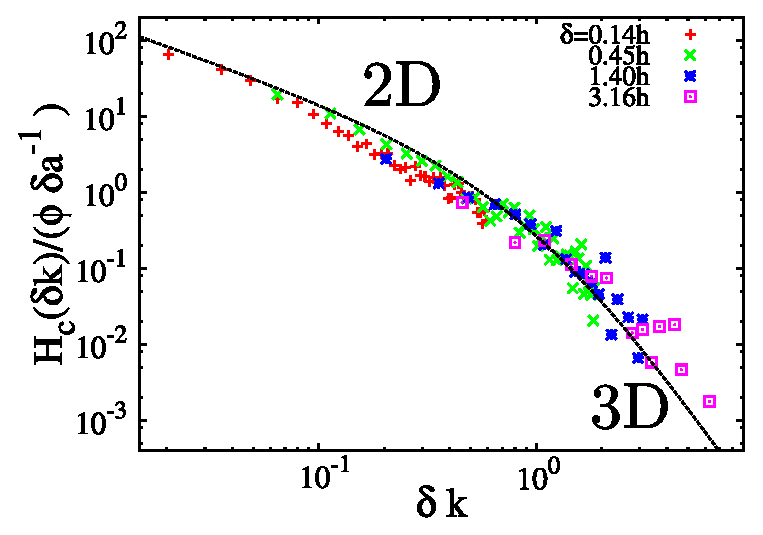
\includegraphics[width=\linewidth]{gfx/q2Dfrom3dto2d}\\
            \end{block}
          }
          \only<3>{\begin{block}{$D_c(k)> 0$ in q2D}          
              \begin{center}
                Correlated density perturbations
                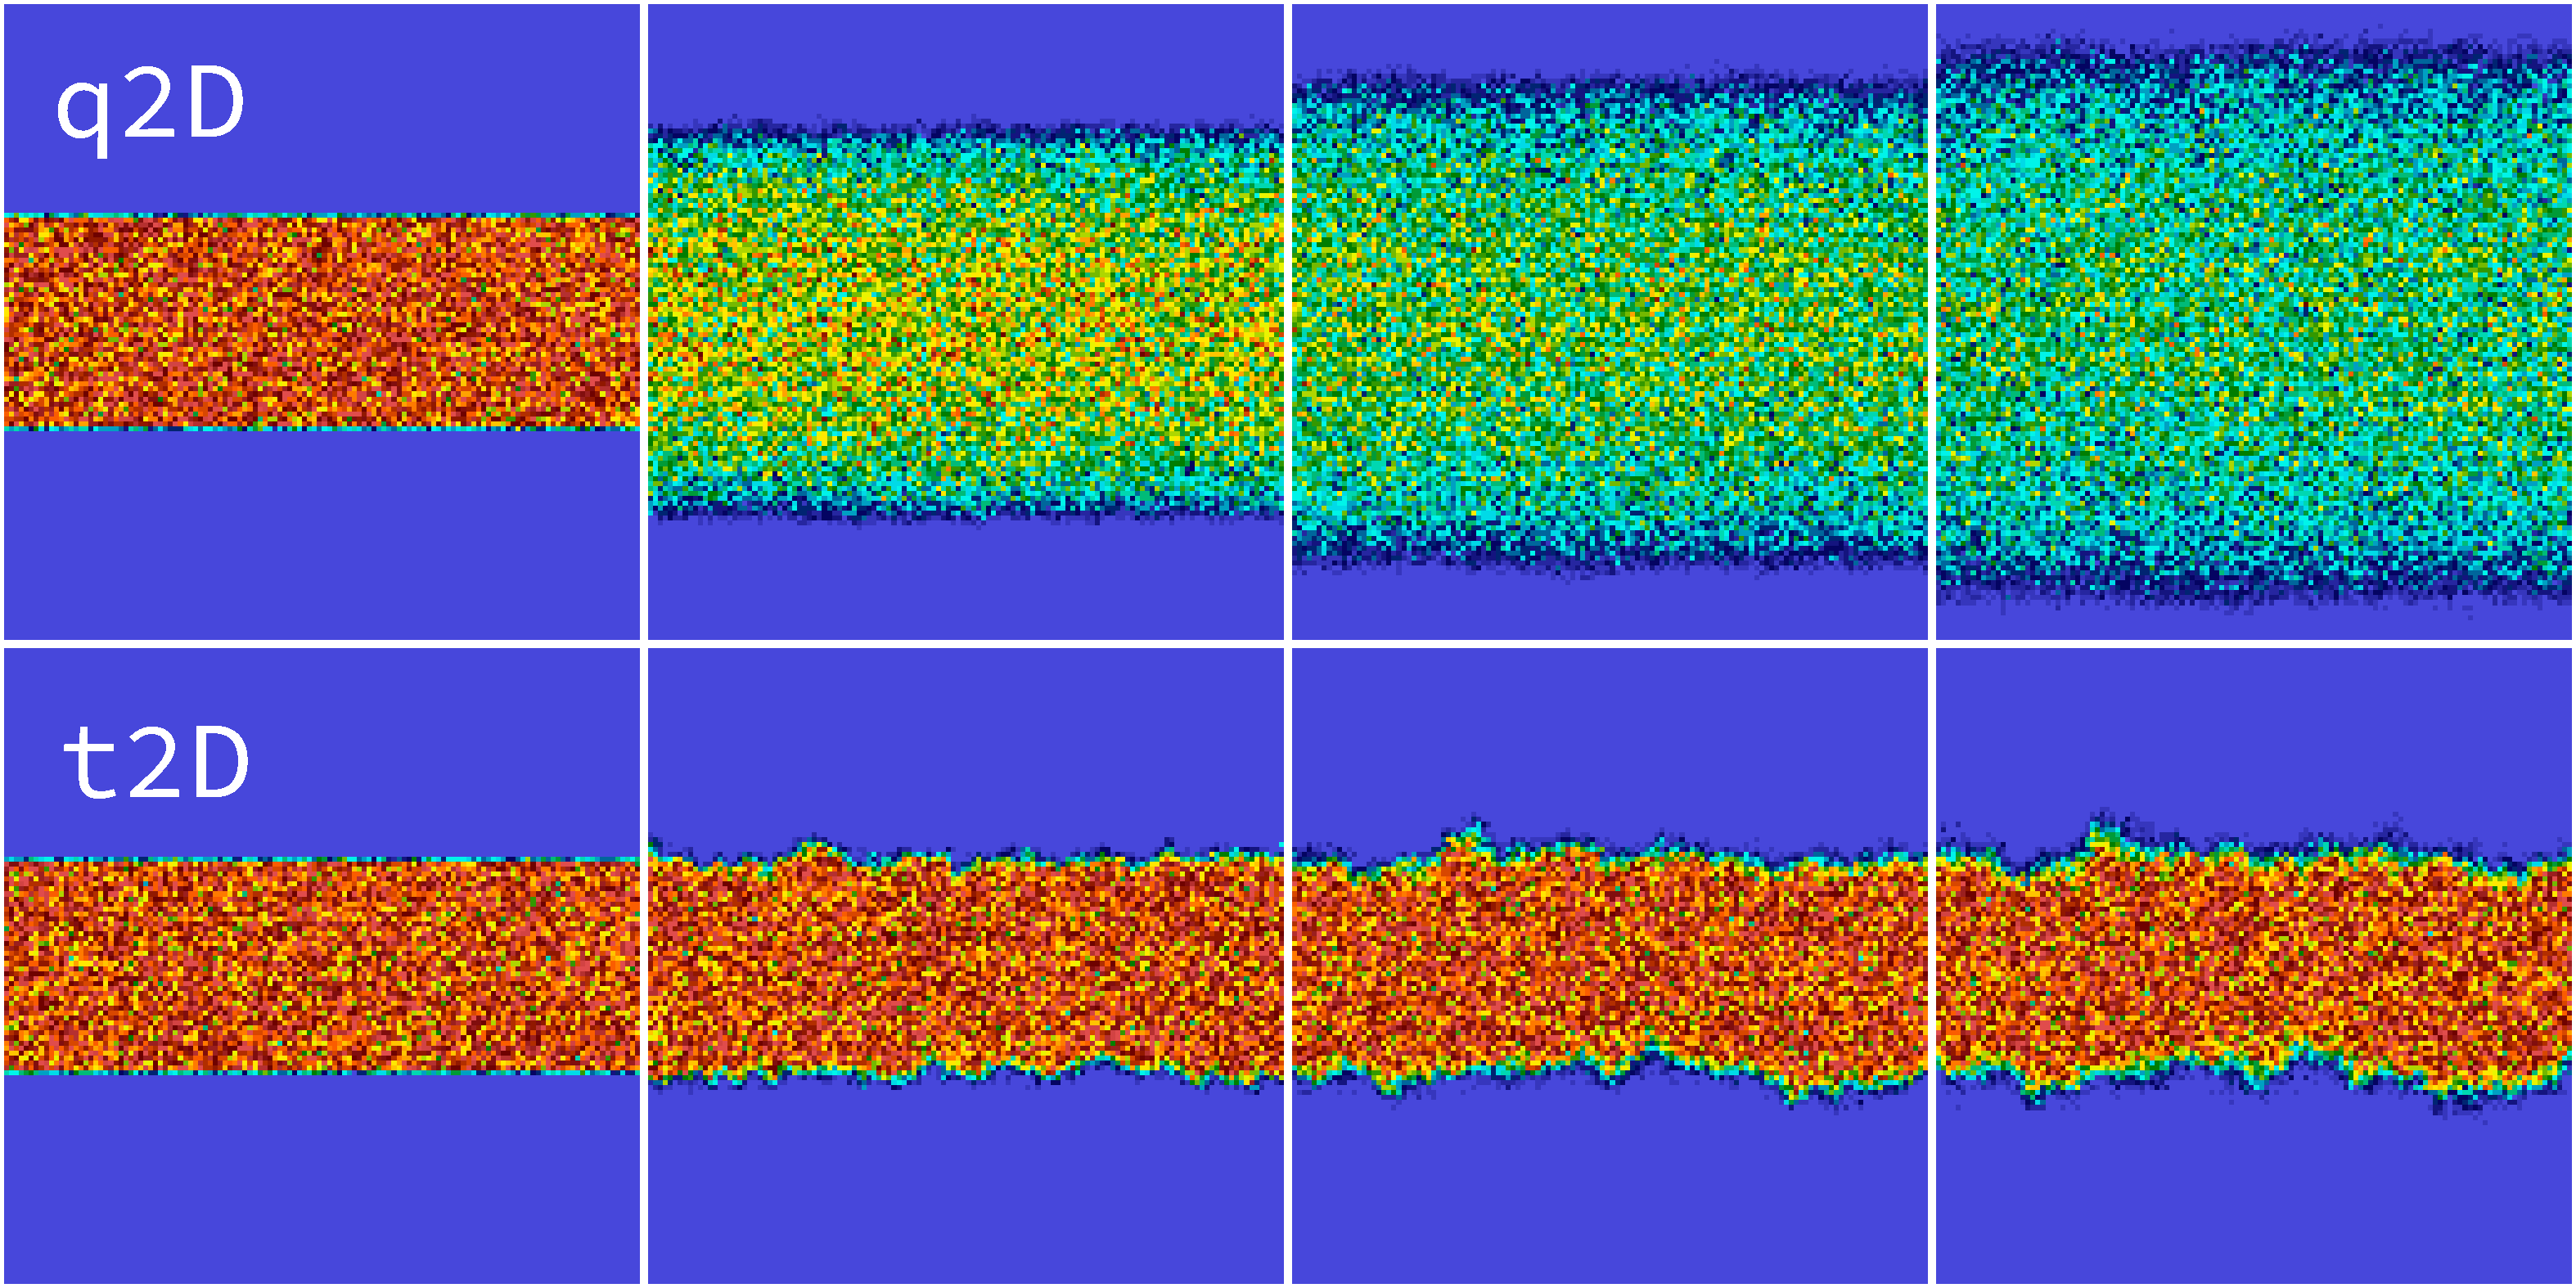
\includegraphics[width=\linewidth]{gfx/q2Dstripes}\\
                \small Time$\rightarrow$
              \end{center}
            t2D: 2D fluid and particles
            \end{block}
          }
        \end{minipage}
      \end{overlayarea}
    \end{column}
  \end{columns}  
  \note<1>{
    \begin{itemize}
    \item Now I want to introduce some modifications to the Force Coupling Method for other kinds of geometries.
    \item I will start with what we call a quasi two dimensional system.
    \item Imagine a fluid that is periodic in the plane but open in the perpendicular direction.
    \item We embed particles in this fluid and confine them with some external potential. The quasi two dimensional limit happens when this force becomes a hard constraint and the particles move strictly in a plane.
    \end{itemize}
  }  
  \note<2>{
    \begin{itemize}
    \item This limit presents a series of abnormal properties that are worth studying. For instance, if we look at the collective diffusion, we see how it diverges with the wave number as we go from an unconfined system to a strictly confined one.
    \end{itemize}
  }
  \note<3>{
    \begin{itemize}
    \item Collective diffusion speaks of the correlation between density perturbations, its divergence in a quasi two dimensional system translates into a drastic enhancement of the dispersion when compared with a fully two dimensional system.
    \end{itemize}
  }
\end{frame}


\begin{frame}
  \frametitle{Force Coupling Method in quasi 2D}
  \begin{overlayarea}{\linewidth}{0.2\paperheight}
    \begin{block}{\centering Force Coupling Method}
      \begin{center}
        \only<1-7>{$\vec{u}_i = \oper{J}_{\vec{\ppos}_i}\mathfrak{F}^{-1}\fou{\oper{G}}_{\text{3D}}(\mathfrak{F}\oper{S}\vec{F} + \vec{k}\cdot\mathcal Z)$}%
        \only<8-9>{$\vec{u}_i = \oper{J}_{\vec{\ppos}_i}\mathfrak{F}^{-1}\left(\fou{\oper{G}}_{\text{3D}}\mathfrak{F}\oper{S}\vec{F} + \fou{\vec{w}}\right)$}
        \only<10-11>{$\vec{u}_i = \oper{J}_{\vec{\ppos}_i}^{\parallel}\mathfrak{F}^{-1}\left(\fou{\oper{G}}_{\qtd}\mathfrak{F}\oper{S}^{\parallel}\vec{F} + \fou{\vec{w}}\right)$}
        \only<12->{$\vec{u}_i = \oper{J}_{\vec{\ppos}_i}^{\parallel}\mathfrak{F}^{-1}\left(\fou{\oper{G}}_{\qtd}\mathfrak{F}\left[\oper{S}^{\parallel}\vec{F} + \vec{\partial}_{\vec{\ppos}}\oper{S}^{\parallel}\left(\kT\right)\right] + \fou{\vec{w}}\right)$}
      \end{center}
    \end{block}
  \end{overlayarea}
  \begin{columns}[T]
    \begin{column}{0.4\linewidth}
      \includesvg[width=0.9\linewidth]{gfx/q2D}\\
      \begin{center}
        q2D: $\delta\rightarrow 0$.\\3D fluid, 2D particles
      \end{center}
      \onslide<11->{
        \begin{equation*}
        \begin{aligned}
        \tens{M}_{\qtd} :=&\oper{J}^{\parallel}\oper{G}_{\qtd}\oper{S}^{\parallel}\\
          \kT \vec{\partial}_{\vec{\ppos}}\cdot \tens{M}_{\qtd} \neq& 0
        \end{aligned}
      \end{equation*}
    }
    \end{column}
    \begin{column}{0.6\linewidth}
      \begin{overlayarea}{\linewidth}{0.7\paperheight}
        \only<1-6>{
          \only<2->{Problems:}
          \begin{enumerate}
          \item<3-> 2D limit implies $F_z\rightarrow \infty$
          \item<4-> Open boundaries in Z require $L_z\rightarrow\infty$
          \end{enumerate}
          \only<5->{Solution:}
          \begin{enumerate}
          \item<6> Eliminate Z direction
          \end{enumerate}
        }
        \only<7-12>{
          Eliminate Z direction:
          \begin{enumerate}
          \item<8-> Fluctuations via FDT
          \item<9-> Preconvolve $\oper{G}$ in Z
          \item<12-> Introduce thermal drift
          \end{enumerate}
        }
        \only<8>{
          \begin{center}
            $\left\langle\fou{\vec{w}}\otimes \fou{\vec{w}}\right\rangle = 2\kT \fou{\oper{G}}$
          \end{center}
        }
        \only<9-12>{
          \begin{block}{Remember}
            $\delta_a(\vec{r}) := \phi(r_x)\phi(r_y)\onslide<9-10>{\phi(r_z)}\rightarrow$ Smeared delta
          \end{block}
        }
        \only<10>{
          \begin{center}
            $\fou{\tens{G}}_{\qtd}(\vec{k}^{\parallel}) = \frac{1}{2\pi}\int\fou{\phi}(k_z)^2\fou{\tens{G}}_{\text{3D}}(\vec{k}^{\parallel},k_z)dk_z$
          \end{center}
        }
        \only<11>{
          \begin{center}
            $\fou{\tens{G}}_{\qtd}(\vec{k}) = \eta^{-1}\left(g(k)\vec{k}^{\perp}\otimes\vec{k}^{\perp} + f(k)\vec{k}\otimes\vec{k}\right)$
          \end{center}
        }
        \only<12>{
          \begin{center}
            $\vec{f}(\vec{r}) = \oper{S}^{\parallel}\vec{F} + \vec{\partial}_{\vec{\ppos}}\oper{S}^{\parallel}[\kT]$
        \end{center}
        }
      \end{overlayarea}
    \end{column}
  \end{columns}
  \note<1>{Let us see how we can adapt the Force Coupling Method to this confined regime.}
  \note<2>{We cannot use triply periodic algorithm directly because in doing so we would have to...}
  \note<3>{...make the confining force infinite}
  \note<4>{And increase the simulation domain to mimic an open boundary.}
  \note<5>{Both of these problems disappear if we eliminate the Z direction from our description.}
  \note<6>{Doing so requires a series of changes.}
  \note<7>{First, lets get fluctuations out of the convolution. We can reintroduce them later ad-hoc with some form that satisfies flucuation-dissipation balance.}
  \note<8>{Now we can use the fact that particles are not allowed to leave the plane and preconvolve them in Z. Remember that the spreading kernel is separable in the three components like this. }
  \note<9,10>{Since the kernel is analytical (in particular we use a Gaussian), and we have the expression of the three-dimensional Greens function, we can simply integrate in the Z direction to get a new Greens function defined only in the plane. Note that spreading and interpolation now happen also in the plane.}
  \note<11>{We end up with a purely two-dimensional description with an analytic form for G. Alas, if we study the mobility, defined as we did before, we see that its divergence, the thermal drift, is different from zero. This speaks of the fact that the flow in the plane is effectively compressible.}
  \note<12>{It is not trivial to show that the thermal drift, that comes from the confining force, appears as an entropic force coming from a pressure gradient and has this particular shape.
    This concludes the adaptation of the Force Coupling method to quasi two-dimensional geometries. And it is worth mentioning that we have some lee-way when choosing the Green's function here, allowing to reuse the same algorithm for other kinds of strongly confined systems. Such as when the fluid is also two dimensional.}  
\end{frame}


\begin{frame}
  \frametitle{Doubly Periodic Force Coupling Method}
  \begin{block}{\centering Stokes equations}
    \begin{overprint}
      \onslide<1-6>
      \begin{equation*}
        \eta \nabla^2\vec{\fvel} =  \nabla \pi - \vec{f}, \qquad   \nabla\cdot\vec{\fvel} = 0%
      \end{equation*}
      \onslide<7->
      \begin{equation*}
        \eta \left(\partial_z^2-k^2\right)\vec{\fou{\fvel}} =
        \begin{bmatrix}
          i\vec{k}\\
          \partial_z
        \end{bmatrix}
        \fou{\pi} - \vec{\fou{f}}, \qquad   [i\vec{k},\partial_z]\cdot\vec{\fou{\fvel}} = 0%
      \end{equation*}
    \end{overprint}
\end{block}
  \begin{columns}[T]
    \begin{column}{0.45\linewidth}
      \begin{minipage}{\linewidth}
        \includesvg[width=1.1\linewidth]{gfx/dpstokes_sketch}
        \only<1>{
          \begin{columns}
            \begin{column}{0.48\linewidth}
              \begin{block}{Fluid forcing}
                \centering $\vec{f}(\vec{r}) = \oper{S}(\vec{r})\vec{F}$
              \end{block}
            \end{column}
            \begin{column}{0.5\linewidth}
              \begin{block}{Particle velocity}
                \centering $\vec{u}_i = \oper{J}_{\vec{q}_i}\vec{v}(\vec{r})$
              \end{block}
            \end{column}
          \end{columns}
        }
      \end{minipage}
    \end{column}
    \begin{column}{0.55\linewidth}
      \only<10->{
        Hardships
        \begin{enumerate}
        \item<11-> BVP solver
        \item<12-> Requires Chebyshev space in Z
          \only<12>{
            \begin{center}
                \includesvg[width=0.6\linewidth]{gfx/chebgrid}
            \end{center}
          }
        \item<13-> Walls added as corrections
          \only<13>{
            \begin{equation*}
              \vec{\fvel}^* = \vec{\fvel} + \vec{\fvel}_{\text{corr}} \rightarrow \vec{\fvel}^*(z=\pm H) = 0 
            \end{equation*}
          }
        \item<14-> Fluct. require iterative solver\\
          \begin{itemize}
          \item Lanczos: $\sim 10$ Stokes solves
          \item Thermal drift: 2 Stokes solves 
          \end{itemize}
        \end{enumerate}
      }
      \begin{overlayarea}{\linewidth}{0.8\paperheight}
        \only<2-5>{Problems:
          \begin{enumerate}
          \item<2-> Unknown Green's function        
          \item<3-> Cannot use $\mathfrak{F}$ in $Z$
          \end{enumerate}    
          \only<4->{Solutions:
            \begin{enumerate}
            \item<4-> Solve Stokes directly
            \item<5-> $\mathfrak{F}$ only in $XY$ plane        
            \end{enumerate}
          }
        }
        \begin{overlayarea}{\linewidth}{0.2\paperheight}
          \only<6-8>{
            \centering $\mathfrak{F}$ only in $XY$ plane
            \begin{equation*}
            \begin{aligned}
              \nabla &\rightarrow \left[ik_x, ik_y, \partial_z\right] := [i\vec{k},\partial_z]\\
              \vec{f} &\rightarrow \left[\fou{f}_x, \fou{f}_y, f_z\right] := \fou{\vec{f}}(\vec{k}, z)
            \end{aligned}
          \end{equation*}
          }
          \only<9>{
            BVP for each $\vec{k}$. Embarrassingly parallel
          }          
        \end{overlayarea}
        \only<8>{
          \begin{equation*}
            \nabla^2\pi = \nabla\cdot\vec{f}
          \end{equation*}
        }
        \only<9>{
          \begin{equation*}
            \begin{aligned}
              \left(\partial_z^2-k^2\right)&\fou{\pi} = \left[i\vec{k}, \partial_z\right]\cdot\fou{\vec{f}}\\
              \onslide<9->{\left(\partial_z \pm k\right)&\fou{\pi}(\vec{k}, z=\pm H) = 0}
            \end{aligned}
          \end{equation*}
        }
      \end{overlayarea}
    \end{column}
  \end{columns}
  \note<1>{
    \begin{itemize}
    \item The quasi two-dimensional framework is based on the assumption that the embedded particles are not allowed to leave the plane. It is of no use if we want to simulate something anisotropic, like a lipid bilayer.
    \item I will now introduce a Force coupling-like method to simulate a doubly periodic domain. That is periodic in the plane and open in the third direction, while having an arbitrary width.
    \item We will again use the same Stokes equations, but changing the boundary conditions requires a lot of rework.
    \end{itemize}
  }
  \note<2>{For starters, we do not know the Green's function, and our previous preconvolution trick does not apply.}
  \note<3>{Boundaries are not periodic in Z, so Fourier is not going to help there.}
  \note<4>{Our solution is to solve the Stokes equation without using the Greens formalism.}
  \note<5>{And the trick lies in Fourier transforming only in the periodic directions.}
  \note<6>{Lets do just that. Now the different quantities depend on a wave vector and a height.}
  \note<7>{And the Stokes equation is transformed into a set of equations independent for each wave vector.}
  \note<8>{There are two unknowns in the Stokes equation: velocity and pressure. But we can use the incompressibility condition to eliminate the pressure.}
  \note<9>{We end up with a set of independent Boundary Value Problems for the pressure (one for each wave vector). Once we have the pressure, we replace it in the Stokes equation and solve for the velocity. Then we transform that velocity back to real space and interpolate to the particles as usual.}
  \note<10>{This is easier said than done, though.}
  \note<11>{Although embarrassingly parallel, the BVP solver is not straight-forward to encode in a GPU.}
  \note<12>{In particular, it involves defining the Eulerian fields in a Chebyshev grid in the Z direction and performing a so-called fast Chebyshev transform, which is similar to a Fast Fourier transform.}
  \note<13>{If we want different boundary conditions, such as no-slip walls, we must add them as a correction.}
  \note<14>{Finally, we only know how to add fluctuations via iterative solvers, which require several Stokes solves. And similarly to the quasi 2D case, we also have to add thermal drift, which involves another couple of solves. All in all, we end up again with a mechanism to transform particle forces to velocities that scales linearly with the number of particles. This time for a doubly periodic environment.}   
\end{frame}


\subsection{Electrostatics}
\begin{frame}
  \frametitle{Triply Periodic Electrostatics}
  \framesubtitle{Force Coupling Method for the Poisson equation}
  \begin{center}
    \begin{minipage}{0.5\linewidth}    
      \begin{block}{Poisson}
        \centering $\varepsilon_0\nabla^2\phi = -f(\vec{r}) = -\oper{S}(\vec{r})\vec{Q}$
      \end{block}
    \end{minipage}
  \end{center}
  \begin{overlayarea}{\linewidth}{0.5\paperheight}
    \begin{columns}[T]
      \begin{column}{0.39\linewidth}
        \begin{block}<2->{Spreading}
          $\oper{S}(\vec{r})\vec{Q} = \sum_i Q_i \delta_a(\vec{\ppos}_i - \vec{r})$
        \end{block}
        \begin{block}<3->{Gaussian sources}
          $\delta_a(\vec{r}) = \frac{1}{(2\pi a^2)^{3/2}} e^{-r^2/(2a^2)}$
        \end{block}        
      \end{column}
      \begin{column}{0.59\linewidth}
        \only<4->{
          \begin{equation*}
            \vec{E}(\vec{\fpos}) = \partial_{\vec{\fpos}}\phi \rightarrow \fou{\vec{E}} = i\vec{k}\fou{\phi}
          \end{equation*}
          \begin{equation*}
            \vec{F}_i = Q_i\oper{J}_{\vec{\ppos}_i}\vec{E}
          \end{equation*}

        }
        \begin{block}<5->{Charges to forces}
          $$\vec{F}_i = Q_i\oper{J}_{\vec{q}_i}\mathfrak{F}^{-1}i\vec{k}\fou{\oper{G}}_P\mathfrak{F}\oper{S}\vec{Q}$$
        \end{block}
        \only<6->{$$\fou{\oper{G}}_P = \frac{1}{\varepsilon_0 k^2}$$}
      \end{column}
    \end{columns}
  \end{overlayarea}
  \onslide<1-3>{\footnotesize Supervector notation. Charges $\vec{Q} := \{Q_1,\dots,Q_N\}$}
  \note<1>{Now I will shift the focus to electrostatics. I want to show you how we can employ our recently our tricks to other equations. In particular, the Force Coupling Method for the Stokes equation has an almost one-to-one simile in the Poisson equation.
  Here I am showing the Poisson equation for the potential of a domain in the presence of a charge density. epsilon is the permittivity of the medium. We will start with triply periodic boundary conditions.}
  \note<2>{This time, instead of spreading forces, we will be spreading particle charges. Which is easier, since are spreading only one value, instead of three.}
  \note<3>{Where we typically model our charges as Gaussian clouds.}
  \note<4>{Then, instead of interpolating velocities, we now interpolate electric fields. Which are trivial to compute once we solve the potential, moreover in Fourier space.}
  \note<5>{In the end, we end up with a mechanism to transform particle charges to particle forces that is quite similar to what we have been seeing up until now.}
  \note<6>{Bonus point, the (triply periodic) Green's function is now much more simple.}
\end{frame}

\begin{frame}
  \frametitle{Doubly Periodic Electrostatics}
  \framesubtitle{Force Coupling Method for the Poisson equation}
  \begin{center}
    \begin{minipage}{0.5\linewidth}    
      \begin{block}{Poisson}
        \only<1-8>{\centering $\varepsilon_0\nabla^2\phi = -f(\vec{r}) = -\oper{S}(\vec{r})\vec{Q}$}%
        \only<9->{\centering $\varepsilon_0(\partial_z^2-k^2)\fou{\phi} = -\fou{f}$}%
      \end{block}
    \end{minipage}
  \end{center}
  \begin{overlayarea}{\linewidth}{0.5\paperheight}
  \begin{columns}[T]
    \begin{column}{0.39\linewidth}
      \begin{center}
        \includesvg[width=\linewidth]{gfx/dppoisson_sketch}
      \end{center}
      \only<2->{
        \begin{equation*}
          \footnotesize
          \begin{aligned}
            &{\color{blue} \varepsilon_0E^z(z = 0)} - {\color{ForestGreen}\varepsilon_bE^z(z=0)} = -{\color{ForestGreen}\sigma_b}\\
            &{\color{blue}\varepsilon_0E^z(z = H)} - {\color{BrickRed}\varepsilon_tE^z(z = H)} = {\color{BrickRed}\sigma_t}
          \end{aligned}
        \end{equation*}
      }
    \end{column}
    \begin{column}{0.59\linewidth}
      \begin{overlayarea}{\linewidth}{0.8\paperheight}
        \only<3-7>{Problems:
          \begin{enumerate}
          \item<3-> Unknown Green's function        
          \item<4-> Cannot use $\mathfrak{F}$ in $Z$
          \end{enumerate}    
          \only<5->{Solutions:
            \begin{enumerate}
            \item<6-> Solve Poisson directly
            \item<7-> $\mathfrak{F}$ only in $XY$ plane        
            \end{enumerate}
          }
        }
        \begin{overlayarea}{\linewidth}{0.2\paperheight}
          \only<8-9>{
            \centering $\mathfrak{F}$ only in $XY$ plane
            \begin{equation*}
              \begin{aligned}
                \nabla &\rightarrow \left[ik_x, ik_y, \partial_z\right] := [i\vec{k},\partial_z]\\
                f &\rightarrow  \fou{f}(\vec{k}, z)
              \end{aligned}
            \end{equation*}
          }
          \only<10->{
            Dielectric jumps $\rightarrow \phi = \phi^*+\phi^c$\\
            Free space ($\varepsilon_0=\varepsilon_b=\varepsilon_t$):
            \begin{equation*}
              \begin{aligned}
                &\epsilon_0\nabla^2\phi^* = -f + \delta(z)\sigma_b + \delta(z-H)\sigma_t\\
                & (\partial_z-k)\phi(\vec{k}, 0) = 0
              \end{aligned}
            \end{equation*}
%            Correction:
%            \begin{equation*}
%              \begin{aligned}
%                &\nabla^2\phi^c = 0\\
%                & \varepsilon_0\partial_z\phi^c(z\rightarrow 0^+) -\varepsilon_b\partial_z\phi^c(z\rightarrow 0^-) = m^b_E
%              \end{aligned}
%            \end{equation*}            
            }
        \end{overlayarea}
      \end{overlayarea}
    \end{column}
  \end{columns}  
\end{overlayarea}
\onslide<1>{\footnotesize Supervector notation. Charges $\vec{Q} := \{Q_1,\dots,Q_N\}$}
\note<1>{And to finish with this section, I want to showcase how we can again use this formalism for a doubly periodic domain. Along with hydrodynamics, we can use these algorithms to model things like ionic channels in a cellular membrane.}
\note<2>{We developed an algorithm for doubly periodic electrostatics, translating the lessons we learned for hydrodynamics. Now instead of no-slip walls we have charged surfaces and permitivity jumps.}
\note<3-7>{We have the same problems as before, and we solve them in the exact same way.}
\note<8>{Eventually, we end up with a BVP that is equivalent to the one we had to solve for the pressure in Stokes.
This algorithm also comes with similar hardships as the Stokes one: We need to solve BVPs, different boundary conditions are added as corrections (which can be quite dense mathematically).}
\end{frame}

%\subsection{UAMMD: A GPU framework for complex fluids}
%\begin{frame}
%  \frametitle{\insertsubsectionnavigation{\linewidth}} 
%  \begin{itemize}
%  \item What UAMMD is and tries to achieve
%  \item ``UAMMD has enabled the community to study hydrodynamics in new systems''
%  \item Not trying to sell UAMMD, just showcase what it can do.    
%  \end{itemize}
%\end{frame}

\section{UAMMD}
\begin{frame}
  \frametitle{Talk outline}
  \tableofcontents[
  sectionstyle=show/shaded,
  subsectionstyle=show/show/hide,
  subsubsectionstyle=show/show/show/hide
  ]
  \note{In this final section I will introduce UAMMD, the GPU software framework for complex fluids that encases, among others, all the algorithms I have previously introduced.}
\end{frame}

\begin{frame}
  \frametitle{The sea of packages}
  \includesvg[width=\linewidth]{gfx/mdpacks}
  \note{UAMMD is born in a crowded sea of molecular dynamics packages. Although most of the commercial packages focus on the microscopic level, in other words, molecular dynamics, many times the limits between molecular dynamics and other descriptions proper to complex fluids is kind of blurred from an algorithmic point of view. So in principle this packages, some of them more than others, can be adapted to other descriptions.}
\end{frame}

\begin{frame}
  \frametitle{What makes UAMMD stand out}
  \Large
  \begin{center}
    UAMMD: A CUDA/C++ library for complex fluids.
    \rule{0.7\textwidth}{1.4pt}
  \end{center}
  \begin{itemize}
  \item<1-> Header only and library-like
  \item<2-> Lightweight with minimal dependencies
  \item<3-> Hackable
  \item<4-> Focus on hydrodynamics
  \end{itemize}
  \note<1>{I would like to lay out some key points that make UAMMD, in my opinion, stand out.
    The first one is that UAMMD is header-only library, as opposed to a monolithic single-binary program.
  This facilitates the use of UAMMD as an accelerator library in other projects. For instance, exposing some of its utilities to python.}
\note<2>{The UAMMD source code is lightweight and, besides an NVIDIA GPU with its required software development kit UAMMD does not depend on any code that is not included in its repository.}
\note<3>{I made UAMMD not only adaptable, but hackable. I tried to reduce internal dependencies to a minimum to encourages users to copy or take away parts of it.}
\note<4>{Finally, there are not a lot of packages out there that put the focus on hydrodynamics and/or complex fluids.}
\end{frame}

\subsection{Universally Adaptable Multiscale Molecular Dynamics}
\begin{frame}[t]
  \frametitle{UAMMD}
  \framesubtitle{Universally Adaptable Multiscale Molecular Dynamics}
  \begin{overprint}
    \onslide<+>
    \centering \huge \bf Universal
    \onslide<+>
    \centering \huge \bf Adaptable
    \onslide<+>
    \centering \huge \bf Multiscale
    \onslide<+>
    \centering \huge \bf Molecular Dynamics
  \end{overprint}
  \begin{columns}[T]
    \begin{column}{0.65\linewidth}
      \begin{overlayarea}{\linewidth}{0.6\paperheight}
        \begin{figure}
          \only<1>{%
            \includesvg[width=0.9\linewidth]{gfx/universally}%
          }%
          \only<2>{%
            \includesvg[width=0.8\linewidth]{gfx/virus}%
          }%
          \only<3>{%
            \includesvg[width=0.8\linewidth]{gfx/scales}%
          }%
          \only<4>{%
            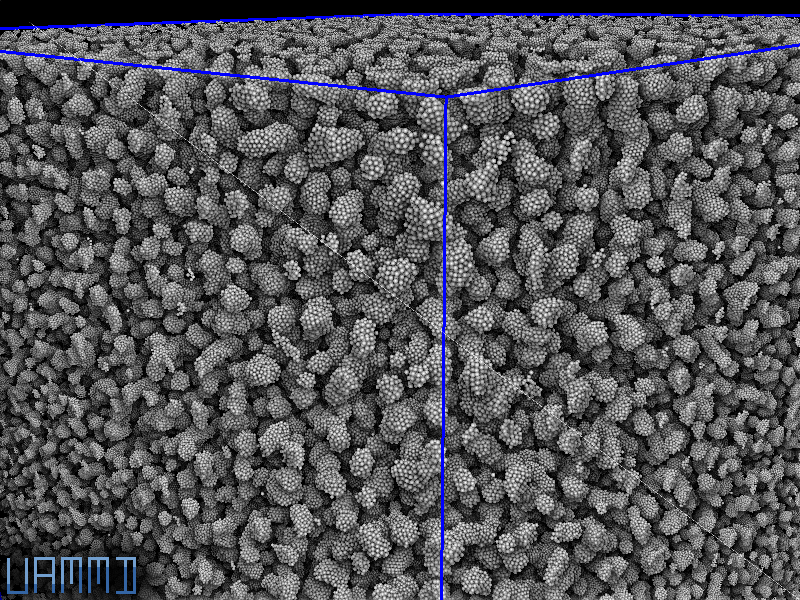
\includegraphics[width=0.9\linewidth]{shotlogo}%
          }%
        \end{figure}
      \end{overlayarea}
    \end{column}
    \begin{column}{0.35\linewidth}      
      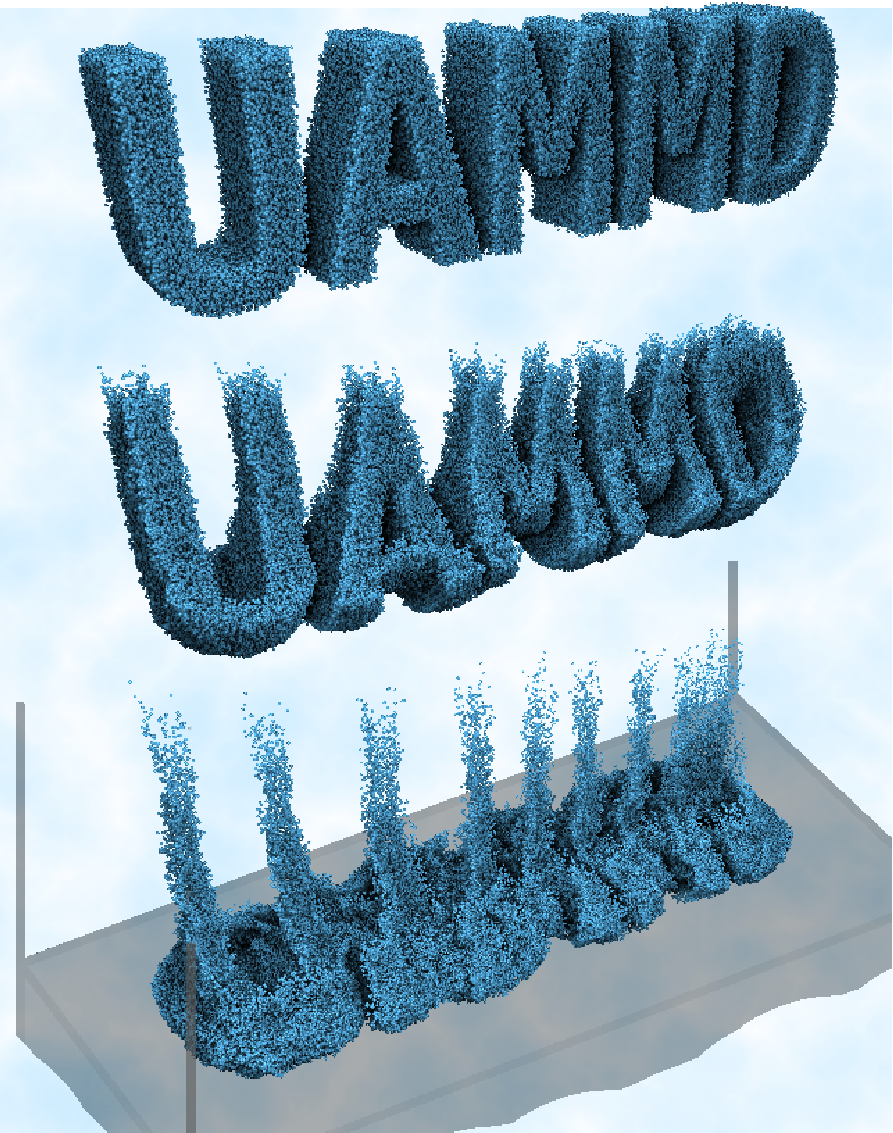
\includegraphics[width=1.0\linewidth]{poster.png}
     \end{column}
   \end{columns}
   \only<1>{\Large Lagrangian and Eulerian descriptions.}%
   \only<2>{\Large Independent building blocks.}%
   \only<3>{\Large Solvers for many scales.}%
   \only<4>{\Large Mainly particle based.}%
   \note<1>{I like to use the UAMMD acronym to introduce its core philosophies. Universal means that both Eulerian and Lagrangian descriptions are supported.}
   \note<2>{Adaptable speaks about the modular design of the code, which I will get into more detail soon. The library is composed of a series of independent modules that can be interconnected to create one simulation or another.}
   \note<3>{Multiscale means that UAMMD offers solvers for all the levels of description that I introduced at the start.}
   \note<4>{Finally, Molecular Dynamics, not the best choice maybe, conveys that particles are the main player. Remember, even when a continuous field, such as a fluid, exists its only as a proxy to communicate the particles.}
\end{frame}
\subsection{Basic code structure}
\begin{frame}[fragile]
  \frametitle{UAMMD}
  \framesubtitle{Conceptual hierarchy}
  \includesvg[width=\linewidth]{gfx/sketchUAMMD}
  \begin{overprint}
    \onslide<1>
    \begin{block}{\centering \Large Remember}
      \centering \Large ``Interacting \emph{particles} with a state that \emph{evolves}''
    \end{block}
    \onslide<2>
    \begin{code2}[]{label=code:module}
      #include<uammd.cuh>
      int main(int argc, char* argv[]){
        auto sys = std::make_shared<System>(argc, argv);
        ...
    \end{code2}
    \onslide<3>
    \begin{code2}[]{label=code:module}
      #include<uammd.cuh>
      int main(int argc, char* argv[]){
        auto sys = std::make_shared<System>(argc, argv);
        const int nP = 1e6; //Number of particles
        auto pd = std::make_shared<ParticleData>(nP, sys);
        ...
      \end{code2}
      \onslide<4>
    \begin{code2}[]{label=code:module}
      ...
      auto pos = pd->getPos(access::cpu, access::write);
      pos[0] = {1,1,1,0}; // x,y,x, color (type)
      ...
    \end{code2}
    \onslide<5>
    \begin{code2}[]{label=code:module}
      ...
      auto md = std::make_shared<VerletNVE>(pd, /*Parameters*/);
      md->forwardTime(); //Exposed by every Integrator
      ...      
    \end{code2}
    \onslide<6>
    \begin{code2}[]{label=code:module}
      ...
      auto elec = std::make_shared<Poisson>(pd,/*Parameters*/);
      elec->sum({.force=true, .energy=false, .virial=false});
      //Exposed by every Integrator
      md->addInteractor(elec);
      md->forwardTime();
      ...      
    \end{code2}
  \end{overprint}
  \note<1>{When introducing complex fluids, I stated that the majority of levels of description in complex fluids can be interpreted as a series of interacting particles with a state that evolves. This sentence is the foundation of UAMMD. A first layer abstracts the actual machine. Then, we enter into a continuous loop that represents a simulation. Particles feed their properties (positions, velocities...) downwards to rest of the modules, and UAMMD distinguishes between two types of modules.
    Integrators, which read the state of the particles at one time and take them to the next. And Interactors, which are used by Integrators to compute Forces, Energies or virials.}
  \note<2>{This conceptual separation is reflected in actual code, where System is a C++ class that can be instantiated.}
  \note<3,4>{In the same way we can initialize an instance of ParticleData, a container for handling the particle properties.}
  \note<5>{Integrators are fed a Particle container and are in charge of forwarding them to the next time step. Integrator is a virtual class, and thus can be specialized for each solver. Here VerletNVE is the UAMMD constant-energy molecular dynamics Integrator.}
  \note<6>{Finally, Interactors, also a virtual class, can be issued to compute forces, etc. and can be added to an Integrator, which in turn will use when forwarding the simulation. Poisson here is the UAMMD Interactor for triply periodic electrostatics.}
\end{frame}
  
\begin{frame}
  \frametitle{Available solvers}
  \includesvg[width=\linewidth]{gfx/sketchUAMMD_integrators}
  \note{This is a list of Integrators available in UAMMD to this date. As you can see, UAMMD exposes solvers for all levels of description that we discussed, and includes Lagrangian and Eulerian/Lagrangian formulations. From molecular dynamics to dissipative particle dynamics and Doubly periodic hydrodynamics.}
\end{frame}

\begin{frame}
  \frametitle{Available interactions}
  \includesvg[width=\linewidth]{gfx/sketchUAMMD_interactors}
  \note{Moreover, the familiar interactions are available as independent Interactor modules, neighbour lists, bonds, electrostatics in several geometries... And the list grows, with collaborators working on Interactors for things like: Optohydrodynamics, magnetism, coarse-grained potentials...}
\end{frame}

\begin{frame}
  \frametitle{UAMMD's online presence}
  \framesubtitle{Git repository}
  {\centering {\color{blue} \url{https://github.com/RaulPPelaez/uammd}}}
  \begin{figure}
    \centering
    \only<1>{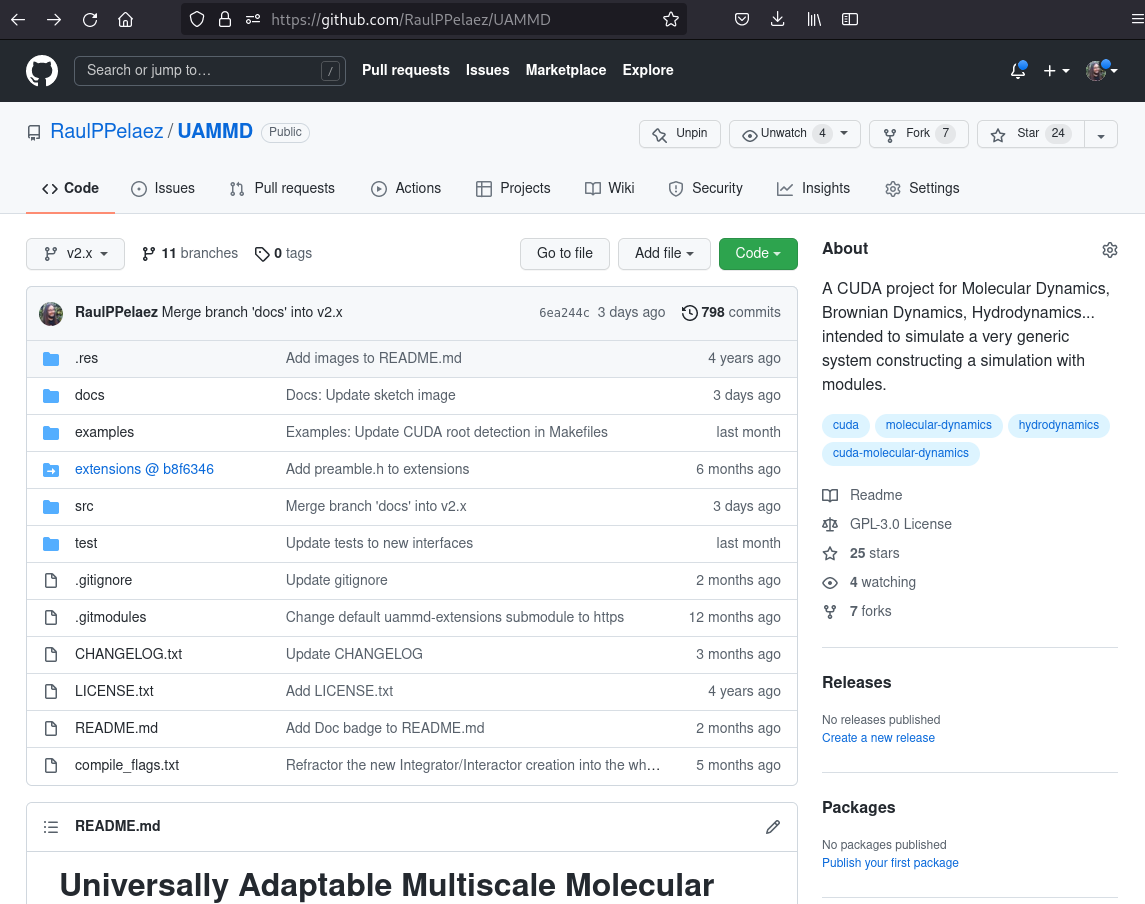
\includegraphics[height=0.7\paperheight]{gfx/uammdgithub}}
    \only<2-3>{
      \onslide<3->{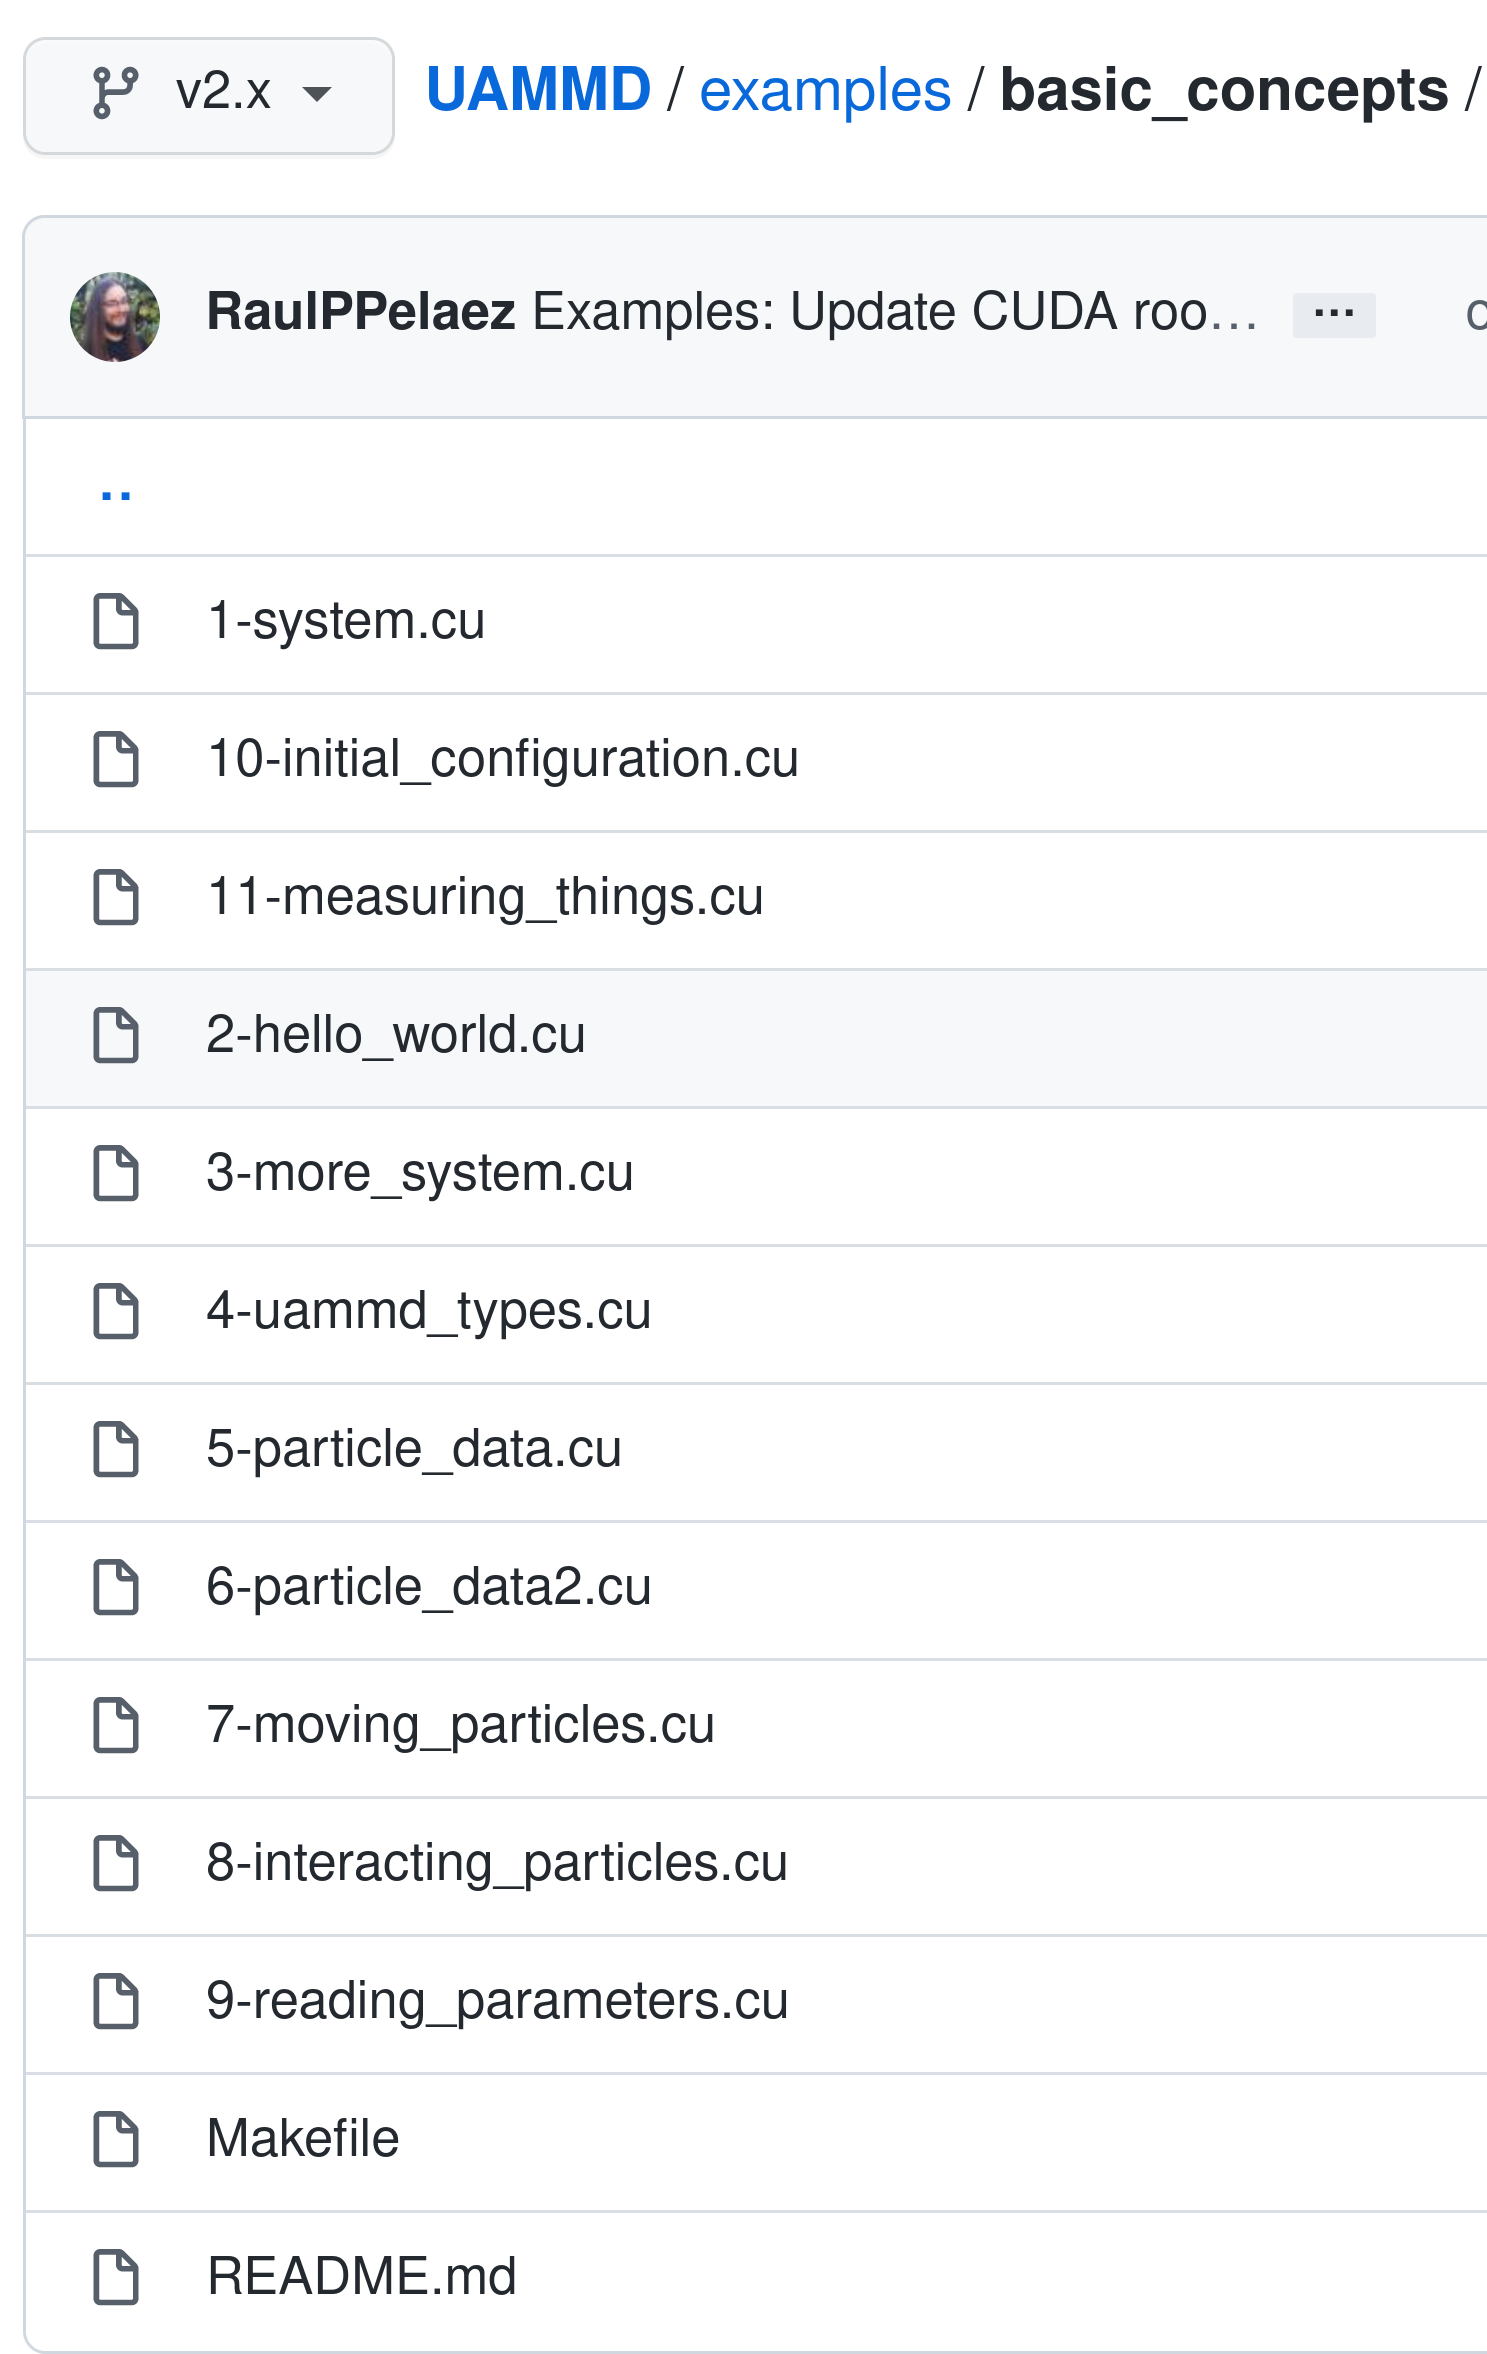
\includegraphics[height=0.7\paperheight]{gfx/uammdtutorial1}}
      \onslide<2->{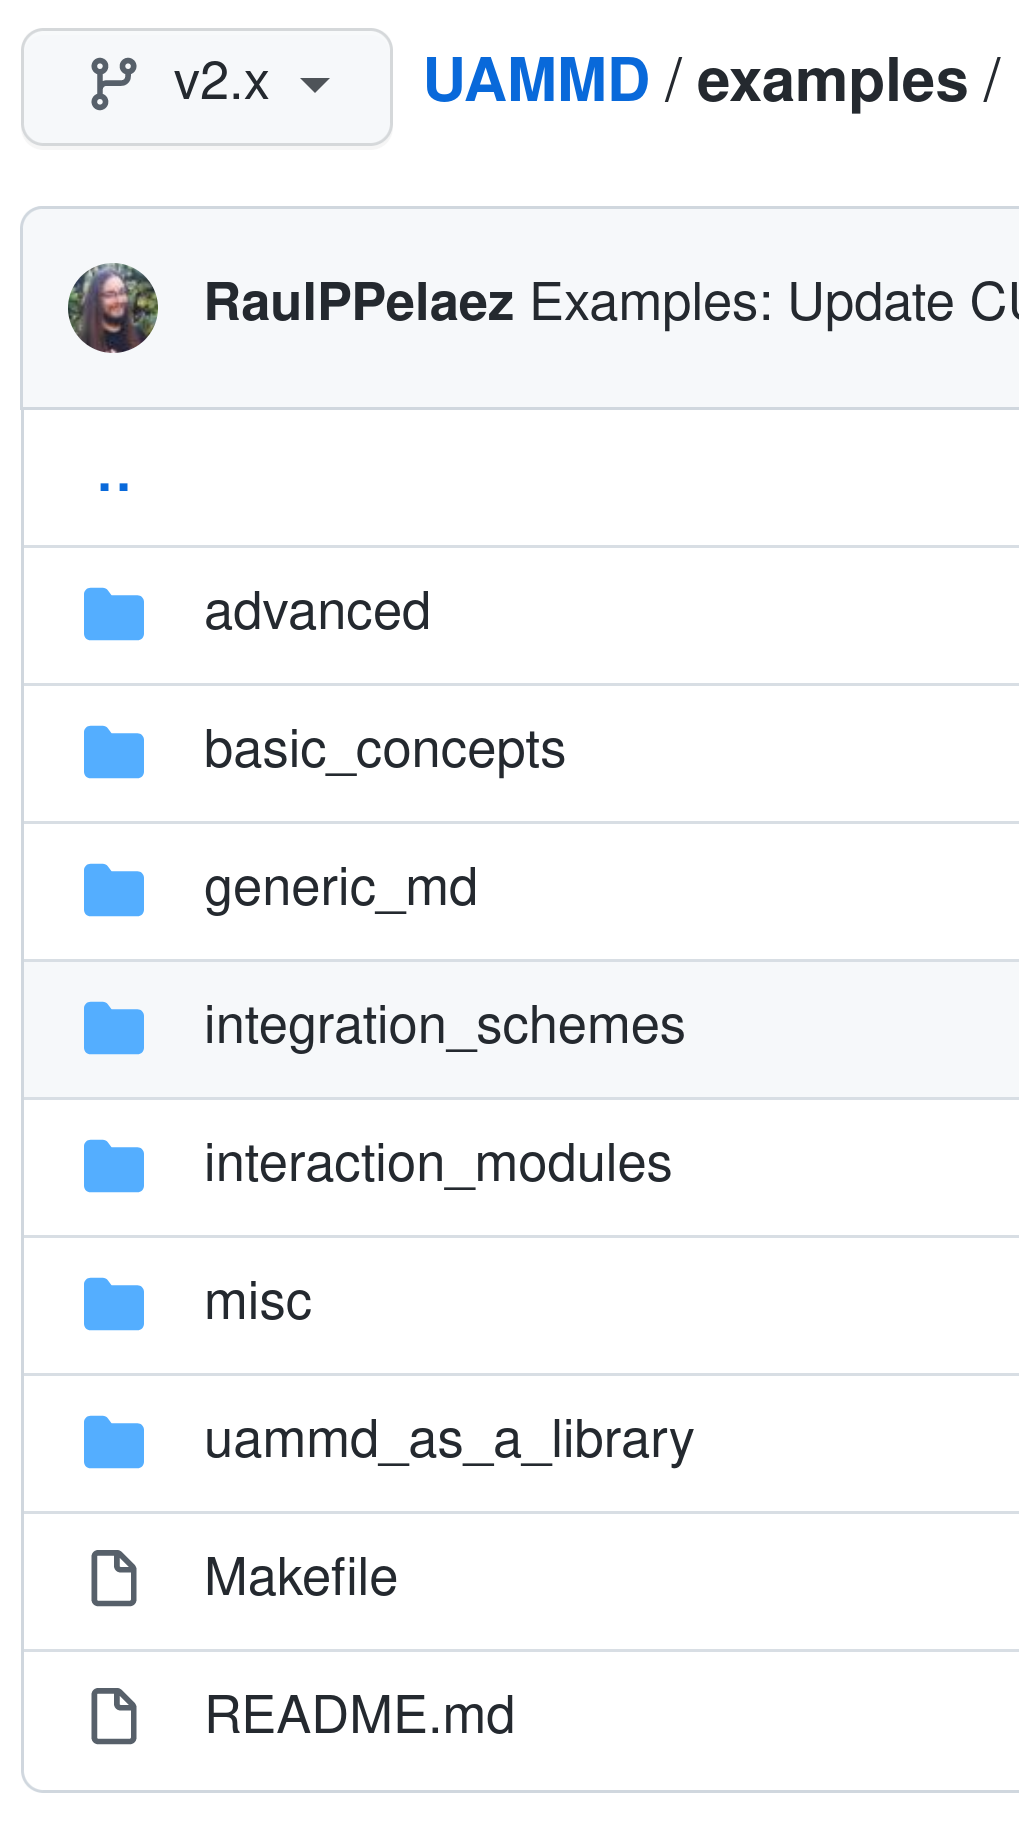
\includegraphics[height=0.7\paperheight]{gfx/uammdexamples}}
    }
    \only<4>{
      \onslide<4->{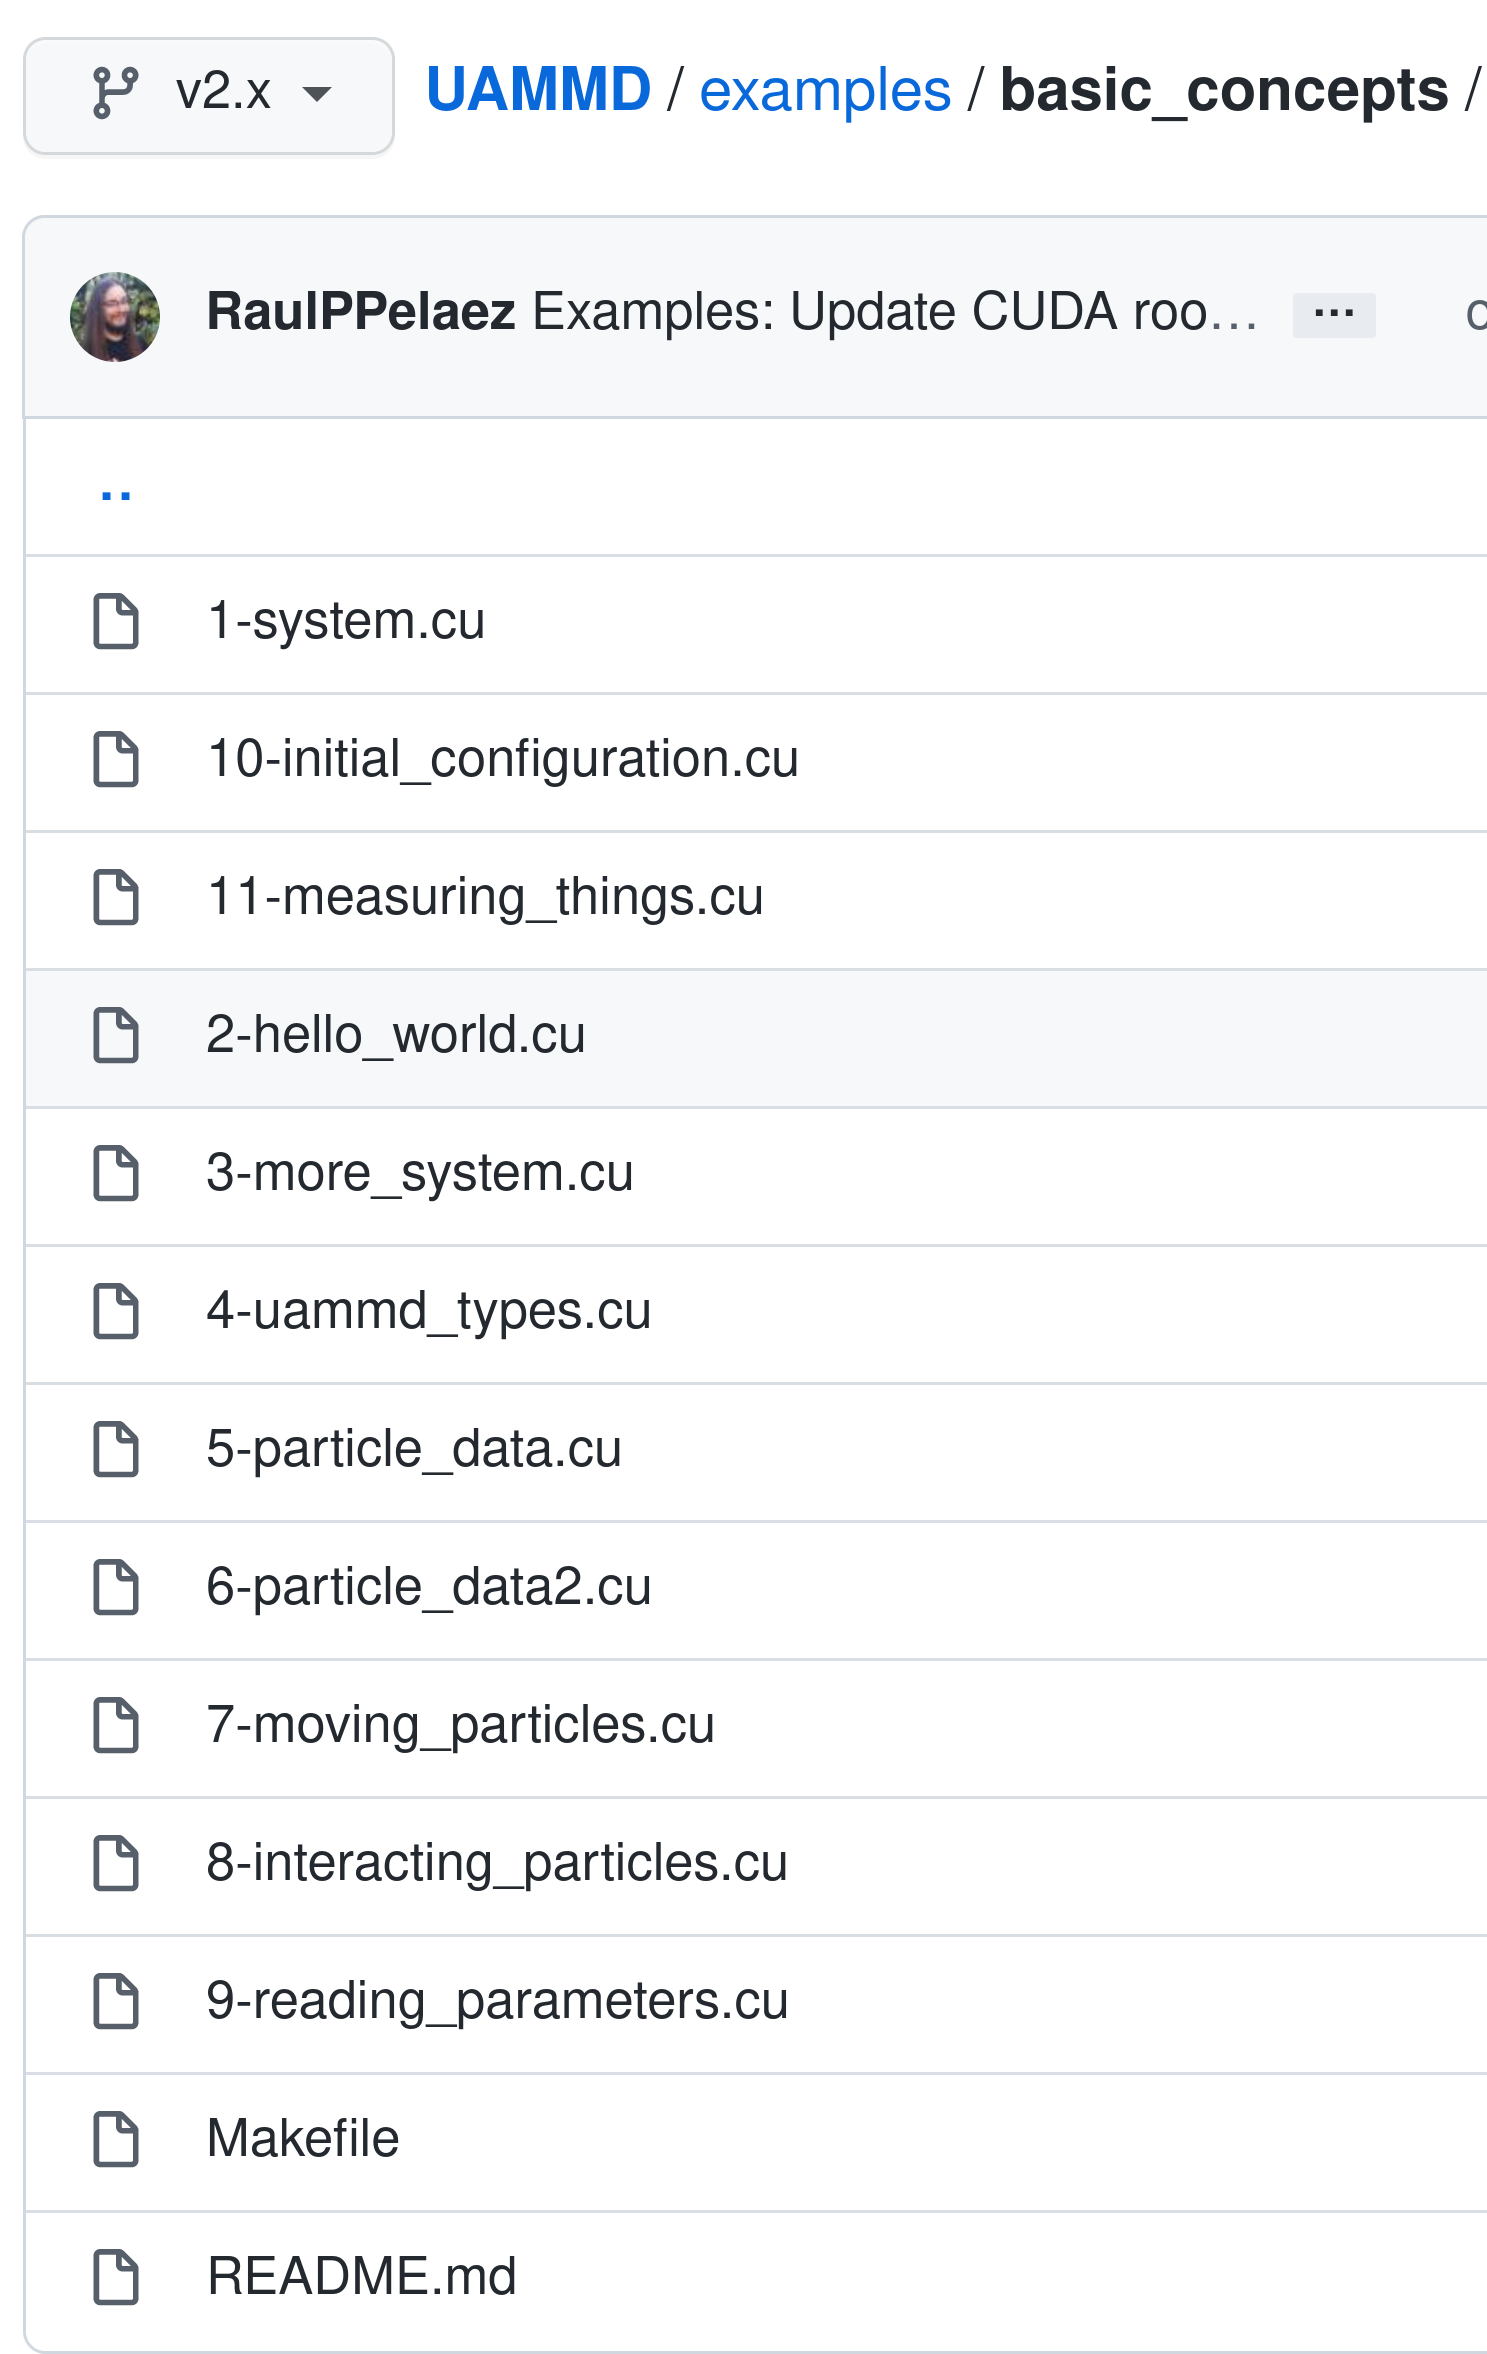
\includegraphics[height=0.7\paperheight]{gfx/uammdtutorial1}}
      \onslide<4->{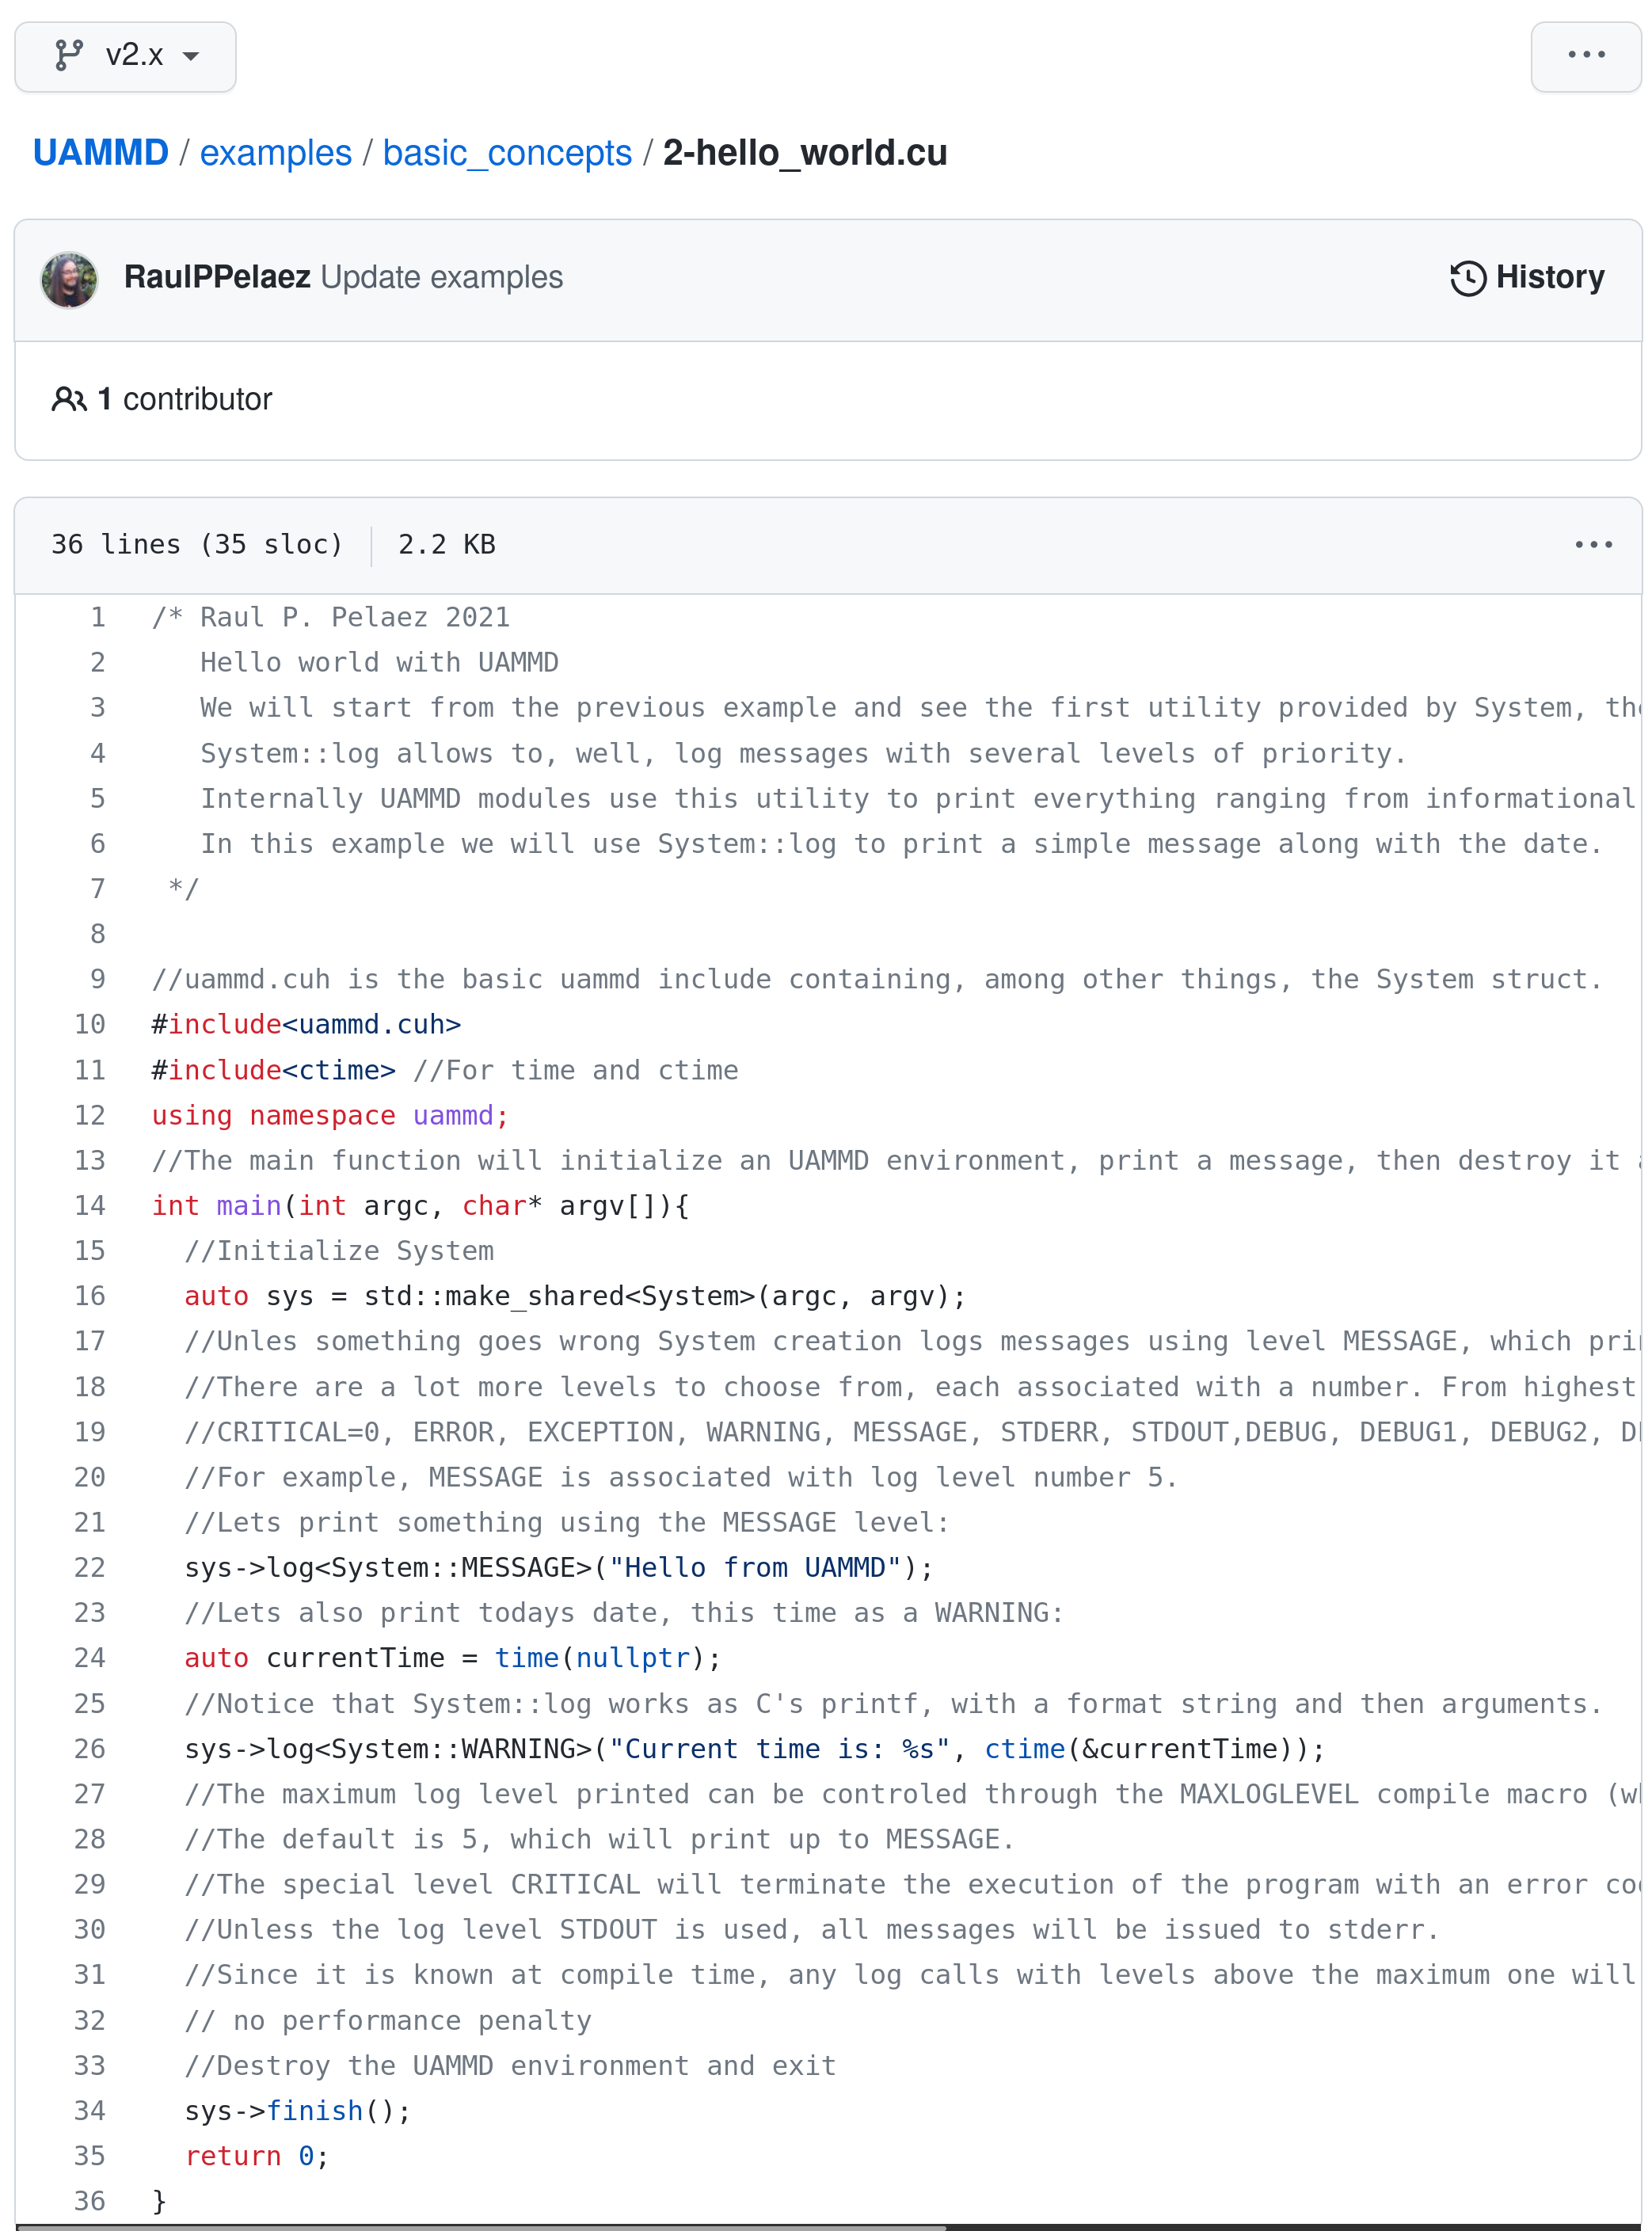
\includegraphics[height=0.7\paperheight]{gfx/uammdtutorial2}}
    }
  \end{figure}
  \note<1>{UAMMD is open-source and freely available as a github repository.}
  \note<2,3,4>{This repository is rich with examples, including an in depth series of them that increasingly introduce the UAMMD concepts in a literary, tutorial fashion.}
\end{frame}

\begin{frame}
  \frametitle{UAMMD's online presence}
  \framesubtitle{Documentation}
  {\centering {\color{blue} \url{https://uammd.readthedocs.io}}}
  \begin{figure}
    \centering
    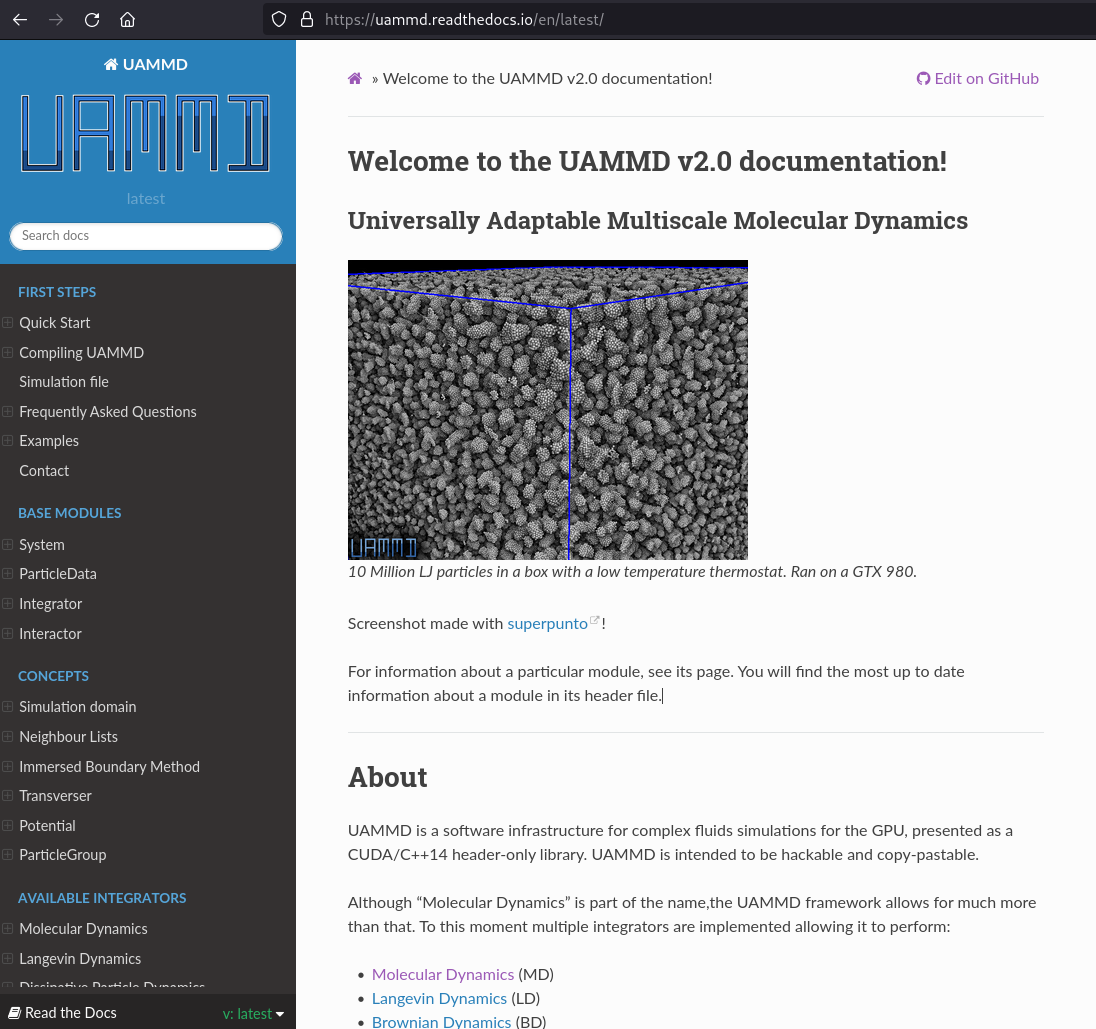
\includegraphics[height=0.7\paperheight]{gfx/uammdreadthedocs}
  \end{figure}
  \only{Finally, a complete documentation is available, with in-depth practical and theoretical information about each existing module and utility in UAMMD.}
\end{frame}

\section{Conclusions}
\begin{frame}
  \setbeamercovered{transparent=40}
%  \setbeamertemplate{itemize/enumerate subbody begin}{\vspace{0.5cm}}
  \setbeamertemplate{itemize/enumerate subbody end}{\vspace{1cm}}
  \frametitle{This thesis main contributions}
  \begin{enumerate}
    \Large\color{blue}
  \item \textbf{Software}.
    \begin{itemize}
    \item<+-> UAMMD: Complex fluids in the GPU      
    \item<+-> Superpunto: A particle visualizator
    \item<+-> GPU post-processing tools: RDF, MSD, correlations...
    \end{itemize}
  \item<+-> \textbf{Algorithms}.
    \begin{itemize}
    \item<+-> Electrostatics and Hydrodynamics in doubly periodic domains.
    \item<+-> Eulerian-Lagrangian coupling.
    \end{itemize}
  \item<+-> \textbf{Physics}.
    \begin{itemize}
    \item<+-> Colloid diffusion under soft (and hard) two-dimensional confinement.
    \item<+-> Dynamics of star-polymer solutions.
    \item<+-> Intra-cellular viscosity.
    \end{itemize}
%  \item Use this slide to give an outline of the talk
  \end{enumerate}
\end{frame}

\end{document}